\documentclass[a4paper,12pt]{report}

\usepackage{alltt, fancyvrb, url}
\usepackage{graphicx}
\usepackage[utf8]{inputenc}
\usepackage{float}
\usepackage{hyperref}

% Questo commentalo se vuoi scrivere in inglese.
\usepackage[italian]{babel}

\usepackage[italian]{cleveref}

\title{Relazione "LiveLand" \\A fun fair simulator}

\author{Valentina Casadei, Enrica Contrini, Livia Del Gaudio, Ines Fraccalvieri}
\date{\today}


\begin{document}

\maketitle
\tableofcontents

\chapter{Analisi}

\section{Requisiti}

Il gruppo si pone come obiettivo quello di realizzare una simulazione interattiva di un parco divertimenti, con la possibilità per l’utente di scegliere come strutturare le attività in esso presenti (variando tra giostre, ristoranti e shop) e il numero di ingressi giornalieri. 
L’applicazione mostrerà gli spostamenti (prevalentemente randomizzati) delle persone nell’ambiente e registrerà le frequenze per ogni attività. L’obiettivo finale sarà quello di mostrare, al termine della simulazione, un’analisi delle attività maggiormente visitate e, nell’ottica di un possibile gestore del parco, statistiche riguardanti gli incassi giornalieri. Successivamente sarà data all'utente la possibilità di salvare l'analisi prodotta su un file a scelta.

\subsection*{Requisiti funzionali}
\begin{itemize}
	\item Organizzazione degli ambienti e delle attività, a scelta dell'utente
	\item Le attività si dividono in Fair (giostre che includono sia quelle per adulti che per bambini) e Profit (attività remunerative, che includono sia negozi che ristoranti).
	\item Al momento dell'ingresso nel parco, le persone vengono generate con età random, sulla base della quale viene loro associato un Ticket. Gli incassi totali derivanti dalla vendita dei biglietti vengono registrati, suddivisi per tipo di biglietto. 
	\item Sulla base dell'età delle persone, vengono effettuati controlli d'accesso nelle giostre, per garantire che i bambini al di sotto dei 12 anni non possano accedere alle giostre per adulti.
	\item Le persone si devono muovere visivamente all'interno del parco, per mostrare ciò che accade al suo interno.
	\item Al termine della simulazione deve essere generata un'analisi su quanto è avvenuto nella simulazione: si prevede di fornire grafici che rappresentino il gradimento delle giostre presenti in percentuale e il totale degli incessi giornalieri suddivisi per attività e per tipo di Ticket.
	\item Una volta generata l'analisi, l'utente deve poter salvare i dati raccolti su un file a scelta.
\end{itemize}

\subsection*{Requisiti non funzionali}
\begin{itemize}
	\item Dal momento che gli spostamenti delle persone saranno prevalentemente randomizzati, sarà necessario utilizzare meccanismi di concorrenza che non impattino eccessivamente sull'utilizzo della CPU durante la simulazione, per garantire la corretta efficienza dell'applicazione.
\end{itemize}

\section{Analisi e modello del dominio}

La simulazione dovrà creare le persone in modo random, associare loro un biglietto generando un PersonTicket e inserirle all'interno dell'Environment. Con Environment si intende la rappresentazione interna del parco, che tiene traccia delle persone che entrano, si muovono ed escono. Il movimento delle persone avviene prevalentemente in direzione delle varie attività presenti. Le attività presenti vengono scelte dell'utente, prima di lanciare il pannello che mostra la simulazione (SimulationPanel), in finestre grafiche apposite (ActivityGui). Le scelte dell'utente circa il setting delle attività nel parco devono essere passate all'EnvironementController, che le aggiungerà nell'EnvironmentActivity, ovvero nella struttura interna del parco.
Le principali challenge da implementare sono la gestione delle persone nel parco, sia per quanto riguarda le entrate/uscite, sia per gli spostamenti: sarà infatti necessario garantire il corretto ricircolo delle persone e il loro movimento allo scorrere del tempo. Successivamente sarà necessario mostrare l'implementazione interna degli eventi nel parco nel pannello della simulazione, dove saranno inserite visivamente anche le attività scelte. Inoltre, un altro punto cruciale sarà capire come rappresentare graficamente i dati raccolti nell'analisi finale, che per il momento si considera solo sotto forma testuale.

\begin{figure}[H]
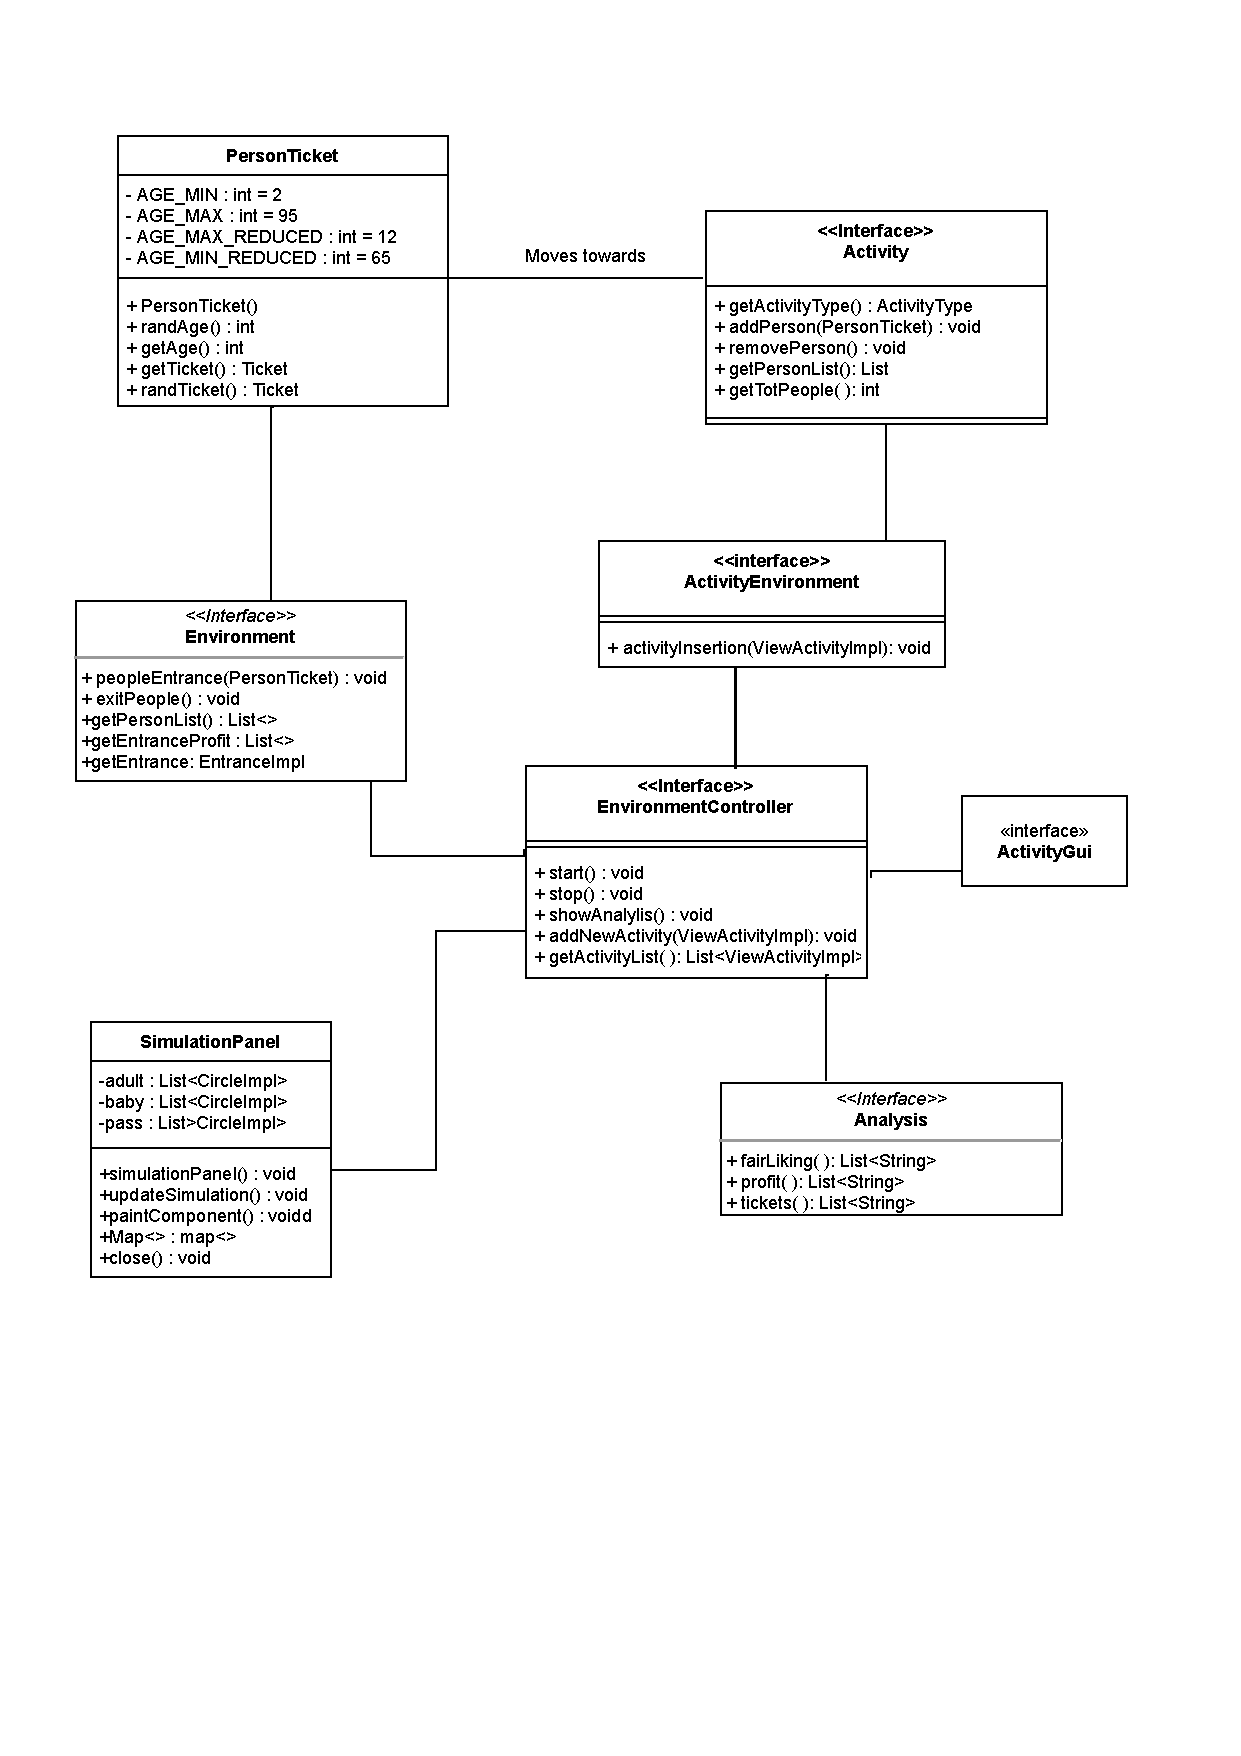
\includegraphics[width=.95\textwidth]{img/analysis.pdf}
\caption{Schema UML dell'analisi del problema, con rappresentate le entità principali identificate ed i rapporti che intercorrono fra loro}
\label{img:analysis}
\end{figure}

\chapter{Design}

\section{Architettura}

L'applicazione LiveLand implementa il pattern architetturale MVC, con l'obiettivo di separare adeguatamente i concetti che appartengono a semantiche diverse. Lo schema principale è quello presentato in Figura 2.1, dove si evidenzia come punto d'accesso all'applicazione la classe Simulator, che istanzia il controller principale, con il compito di settare la View e l'EnvironmentController. La view iniziale ha il compito di richiedere all'utente di inserire i campi per creare le attività, che passeranno attraverso il controller per essere effettivamente istanziate nel Model EnvironmentActivity.\\

\begin{figure}[h]
\centering{}
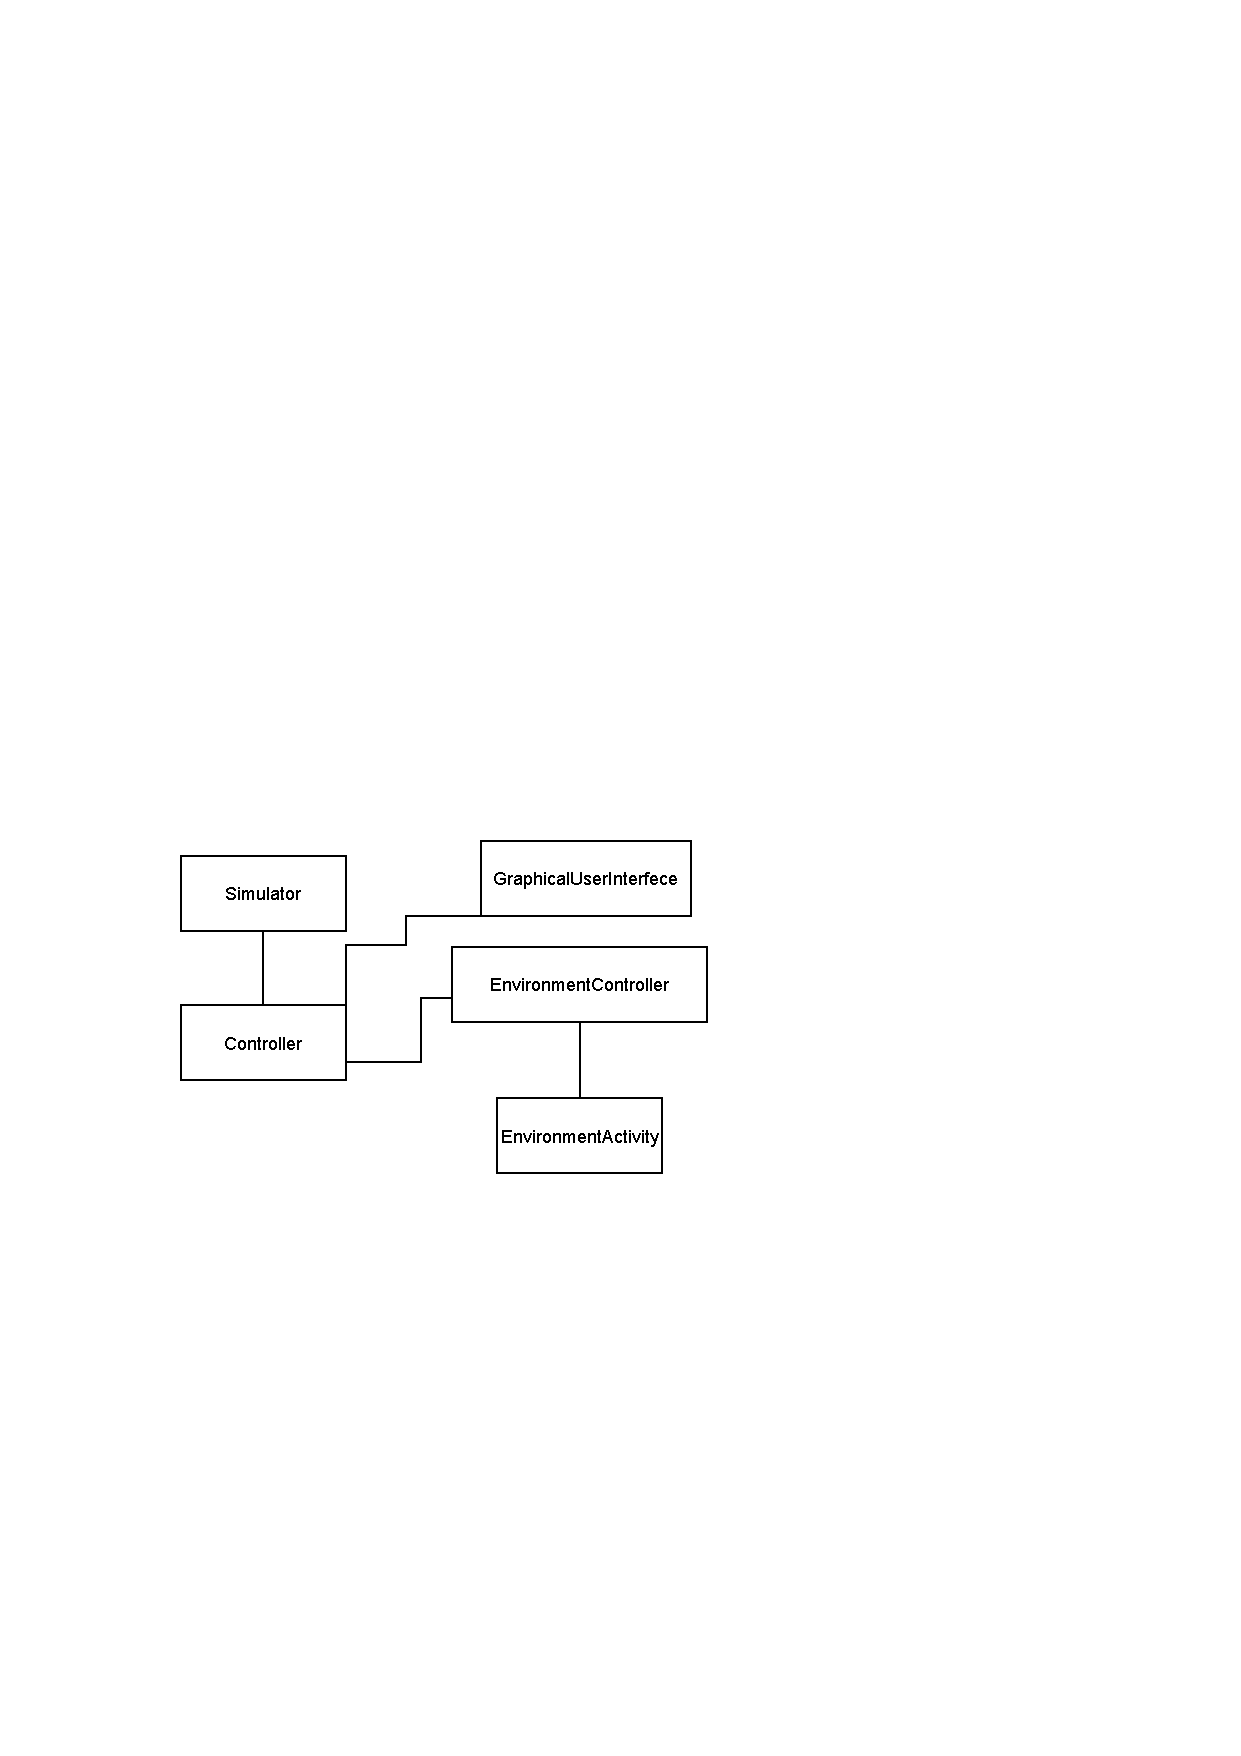
\includegraphics[width=.7\textwidth]{img/arch.pdf}
\caption{Schema UML architetturale di LiveLand, che rappresenta il punto di entrata per il pattern MVC.}
\label{img:arch}
\end{figure}

\paragraph{}Una sostituzione in blocco della View non dovrebbe impattare l'architettura di Model e Controller, poichè le parti di logica sono incapsulate nel model e il controller si occupa solo di fare da "tramite" tra gli altri due elementi. Infatti, con questa architettura, può essere aggiunto un numero variabile di attività, anche se l'aggiunta di un nuovo tipo di attività implicherebbe la necessità di apportare modifiche nel Model.\\\\\\\\


\onecolumn
\section{Design dettagliato}

\paragraph{Valentina Casadei}
Il mio obiettivo all’interno del gruppo riguardava la creazione delle attività e la visualizzazione grafica delle attività.

Per lo sviluppo delle attività ho creato un’interfaccia che viene implementata dalle due classi Fair e Profit che sono le classi dove vengono specificati i metodi delle seguenti attività.

\begin{figure}[h]
\centering{}
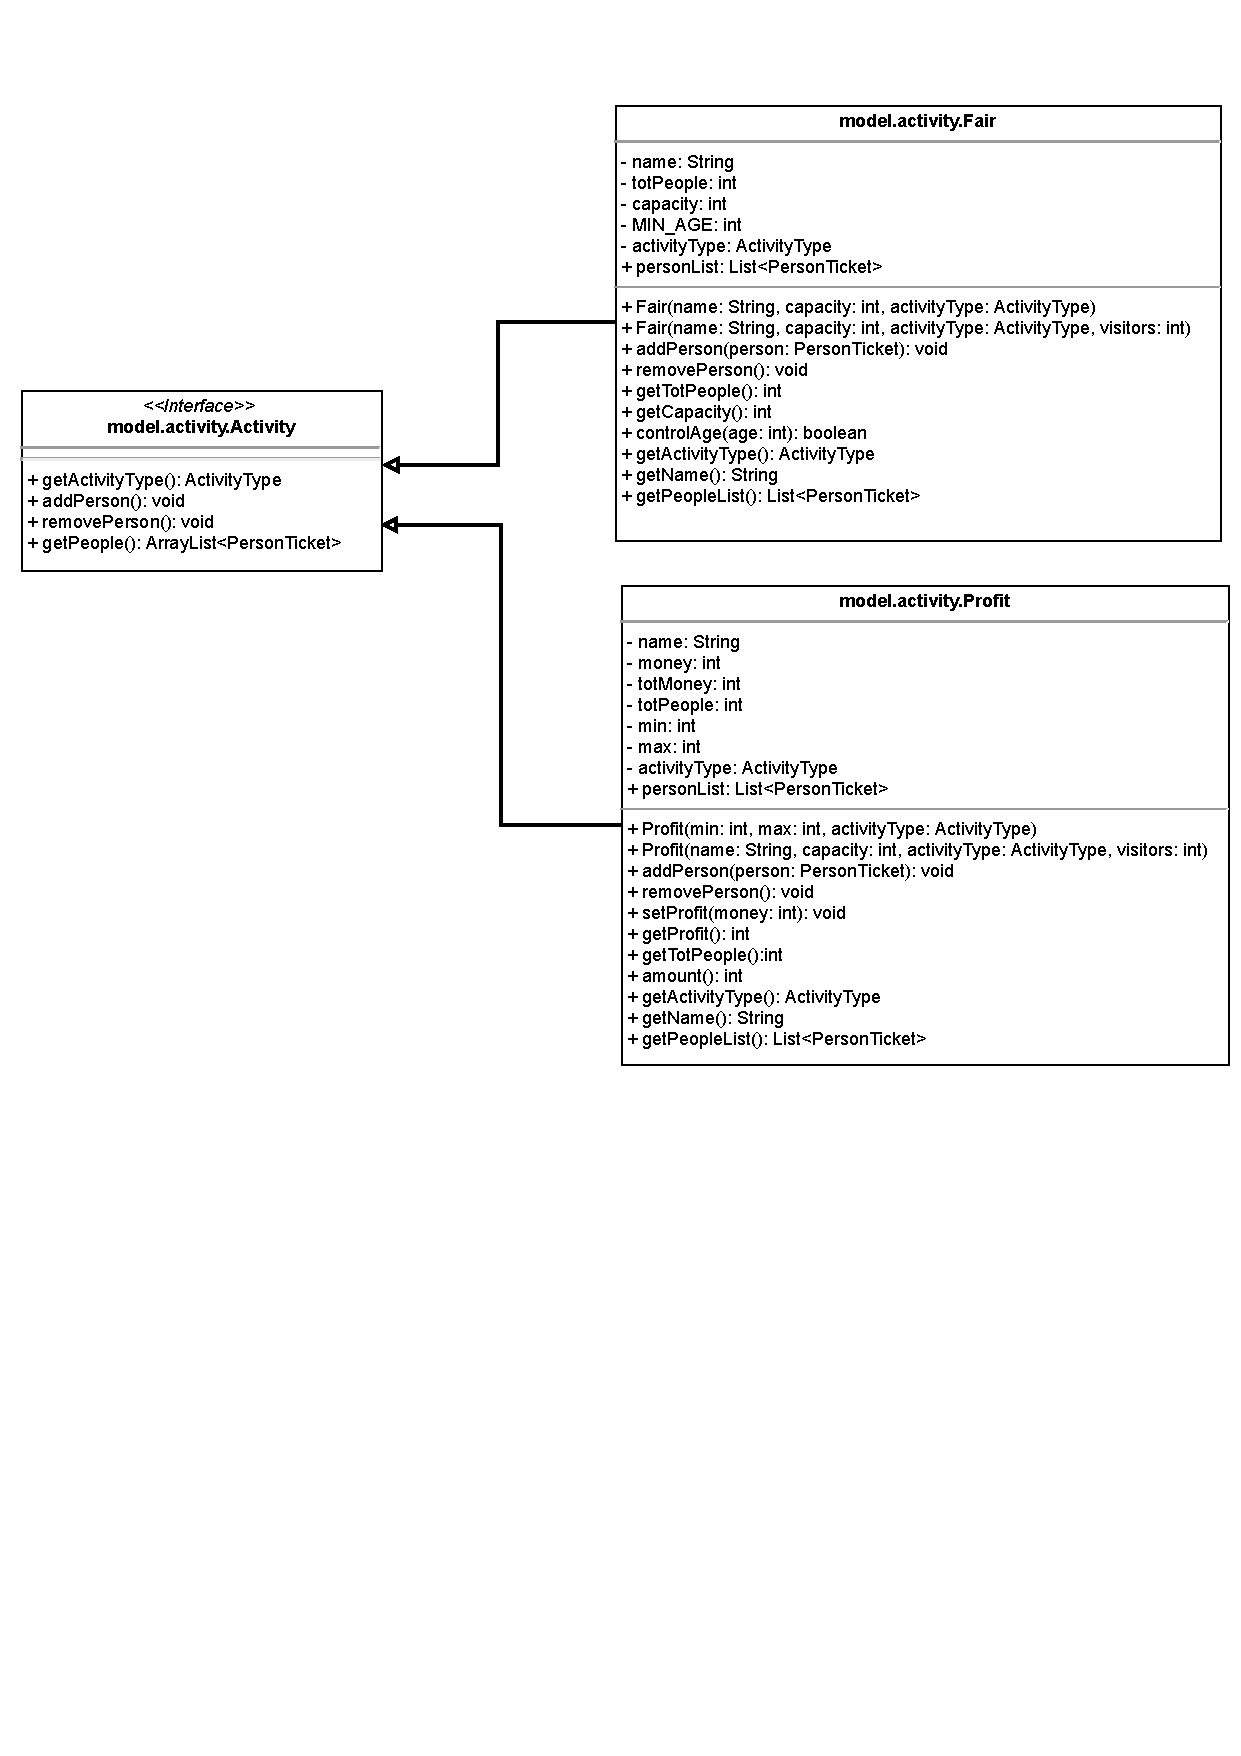
\includegraphics[width=.7\textwidth]{OOP-LiveLand/img/activity.pdf}
\caption{Schema UML rappresentativo del pattern model activity}
\label{img:activity}
\end{figure}

Le attività sono di due tipi: le giostre, le quali si suddividono in giostre per adulti e in giostre per tutti, e i profit i quali si suddividono a loro volta in shop e ristoranti. Ogni attività ha un nome che viene digitato dall’ utente.
In tutte le attività ho gestito l’ingresso e l’uscita delle persone con una lista. Ad ogni singola corsa vengono aggiunti gli oggetti PersonTicket alla lista che poi al termine della corsa verranno rimossi. Ogni volta che la corsa termina verrà memorizzato il numero di persone che sono state ad ogni singola attività.
Le giostre a differenza dei profit hanno la capacità, cioè un numero massimo di persone che possono entrare in ogni singola giostra. La capacità viene digitata dall’utente per ogni singola giostra.
Nei profit invece, abbiamo il guadagno, ad ogni persona gli viene assegnata una spesa random, dove il massimo e il minimo della spesa viene scelto dall’utente. Poi viene tenuto in memoria il guadagno totale delle attività profit. 

Per la creazione della grafica delle attività ho sviluppato una classe Square dove vengono dichiarate le proprietà delle attività. Nella classe DesignActivity creo le quattro attività di tipo Square. Nella classe ActivityInsertion invece faccio un controllo della lista delle attività per sapere quante attività devo rappresentare nel pannello e poi queste attività le inserisco in quattro liste diverse dividendole in base alla loro tipologia. Inoltre, ho inserito nella classe SimulationPanel un ciclo per rappresentare ogni singola lista e disegnare le varie attività.

\begin{figure}[h]
\centering{}
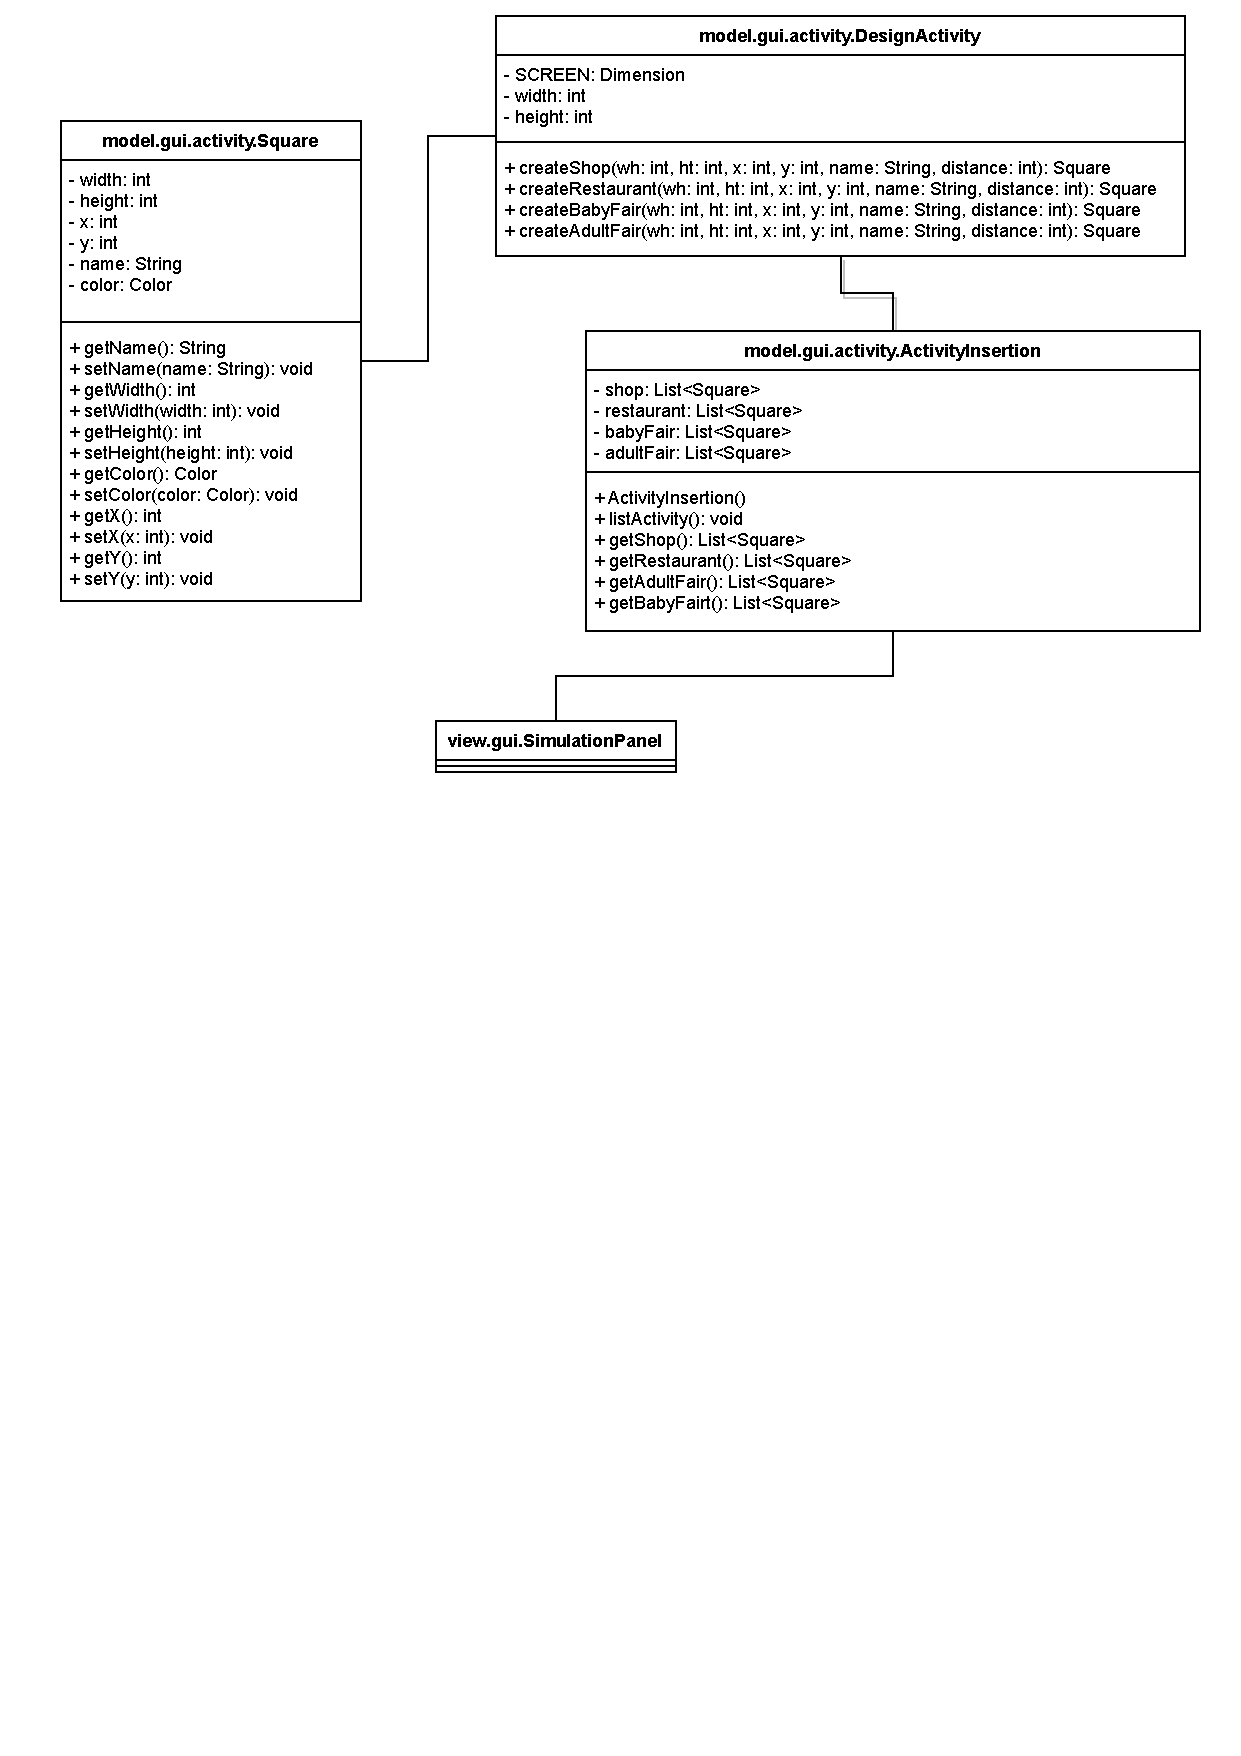
\includegraphics[width=.7\textwidth]{OOP-LiveLand/img/activity_graphics.drawio.pdf}
\caption{Schema UML rappresentativo del pattern model gui activity.}
\label{img:activity_graphics}
\end{figure}

La mia parte grafica consiste nel rappresentare graficamente le attività e disporle nel pannello.
Le attività sono rappresentate con dei rettangoli di quattro colori diversi in base alla loro tipologia. Sopra a tale rettangolo c’è scritto il nome della attività che viene inserito dall’utente nel pannello iniziale. 
Per posizionare i rettangoli ho usato le coordinate x e y. Ho posizionato ogni tipologia di attività in un lato diverso del pannello. Nel lato sinistro si possono trovare gli shop, in basso si possono trovare i ristoranti, in alto le giostre dove quelle più a sinistra sono quelle dove possono andare tutti e quelle più a destra sono quelle per gli adulti. Le attività possono stare fino ad un determinato numero, altrimenti escono fuori dal pannello oppure si sovrappongono.
Le dimensioni delle attività le ho messe in proporzione con lo schermo del computer, in modo da adattarsi a qualsiasi schermo. 

\paragraph{Divisione in package:} Il package model.activity contiene l’interfaccia e le classi relative alla creazione delle attività. Il model.gui.activity contiene le classi relative al posizionamento e alla rappresentazione grafica delle attività.


\paragraph{Enrica Contrini}
\paragraph{Problema} Visualizzazione grafica delle persone nel parco.
\paragraph{Soluzione}Simulationpanel è la classe main che si occupa di creare il pannello principale per la simulazione e di disegnare le attività e le persone.
Vengono create tre liste collegate alle tre tipologie di biglietti: biglietto intero(adult), biglietto ridotto(baby) e abbonamento(pass) che poi verranno disegnati dal paintComponent.
CircleImpl implementa l’interfaccia Circle e serve per creare i cerchi che rappresentano le persone. In questa classe vengono usati i setter e getter che permettono di leggere e assegnare il valore del cerchio. Il getRadius() assegna il raggio del cerchio mentre il getColor() assegna il colore.

\begin{figure}[h]
\centering{}
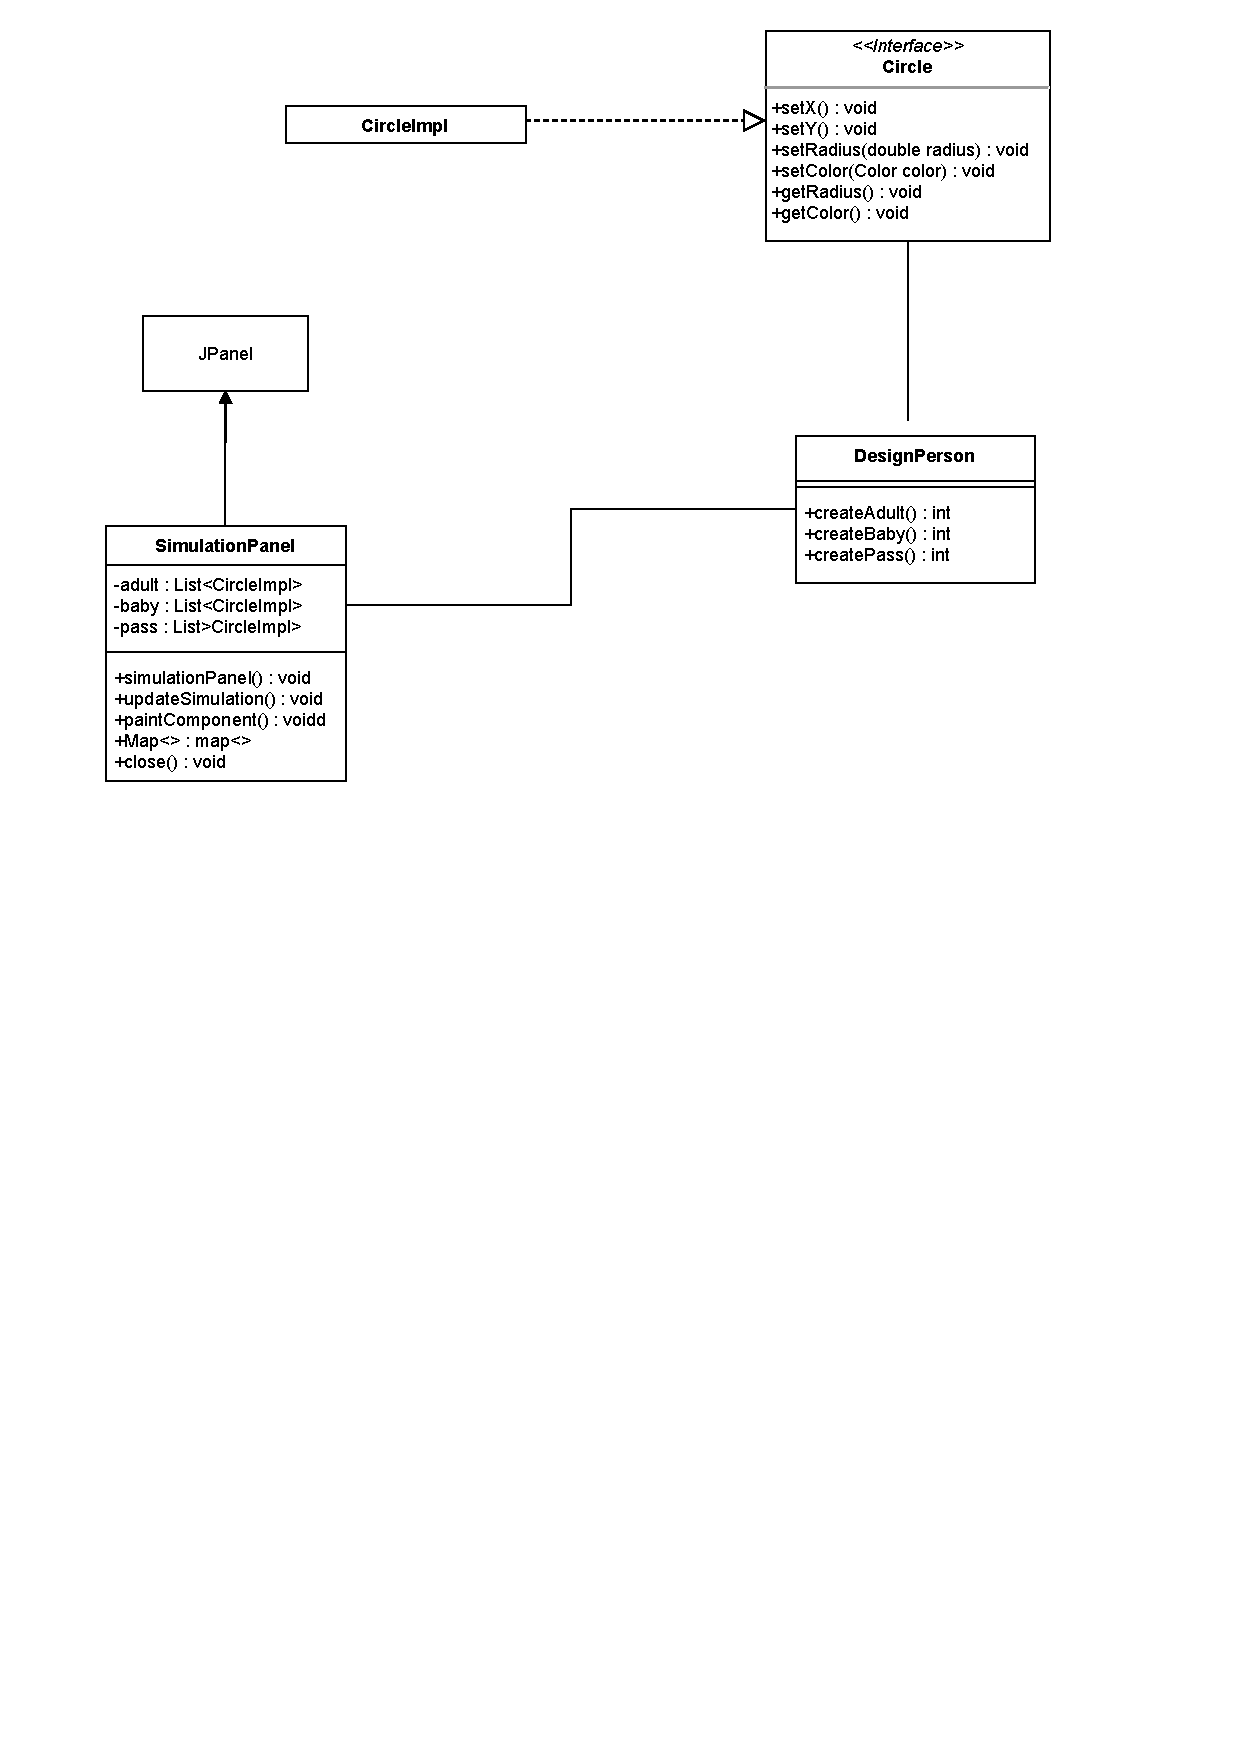
\includegraphics[width=.6\textwidth]{OOP-LiveLand/img/People_GUI.pdf}
\caption{Schema UML della rappresentazione grafica delle persone presenti nel parco.}
\label{img:People_GUI}
\end{figure}

\paragraph{Problema} Implementazione del pattern MVC applicato alla simulazione grafica: gestione del repaint delle ersone allo scorrere del tempo.
\paragraph{Soluzione} Questo è in generale il pattern MVC(model-view-controller). Il Model è rappresentato da Repaint e da Position. Il controller, cioè ViewController riceve i comandi dall’utente attraverso la View ed esegue delle operazioni che possono interessare il Model e che portano ad un cambiamento di stato nel View quindi nel SimulationPanel. 

\begin{figure}[h]
\centering{}
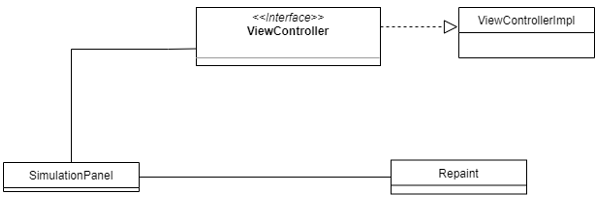
\includegraphics[width=.7\textwidth]{OOP-LiveLand/img/MVC.png}
\caption{Schema UML del pattern MVC applicato alla rappresentazione grafica delle persone nel parco.}
\label{img:MVC}
\end{figure}

\paragraph{Problema} Rappresentare dinamicamente la posizione delle persone all'interno del parco ad ogni istante.
\paragraph{Soluzione} Per determinare la posizione delle persone all'interno del parco una volta entrate viene utilizzata la classe RandomPosition, che assegna una posizione iniziale randomizzata. Successivamente, sulla base delle attività in cui si spostano le persone secondo il thread principale, le posizioni vengono costantemente aggiornate dal metodo RepaintPeople, per poi ridisegnare graficamente le persone nel pannello della simulazione. Per tenere traccia delle persone e delle posizioni correnti, viene usata una mappa in cui la chiave è rappresentata dal PersonTicket, mentre il valore associato è la posizione corrente, che sarà di volta in volta aggiornata.

\begin{figure}[h]
\centering{}
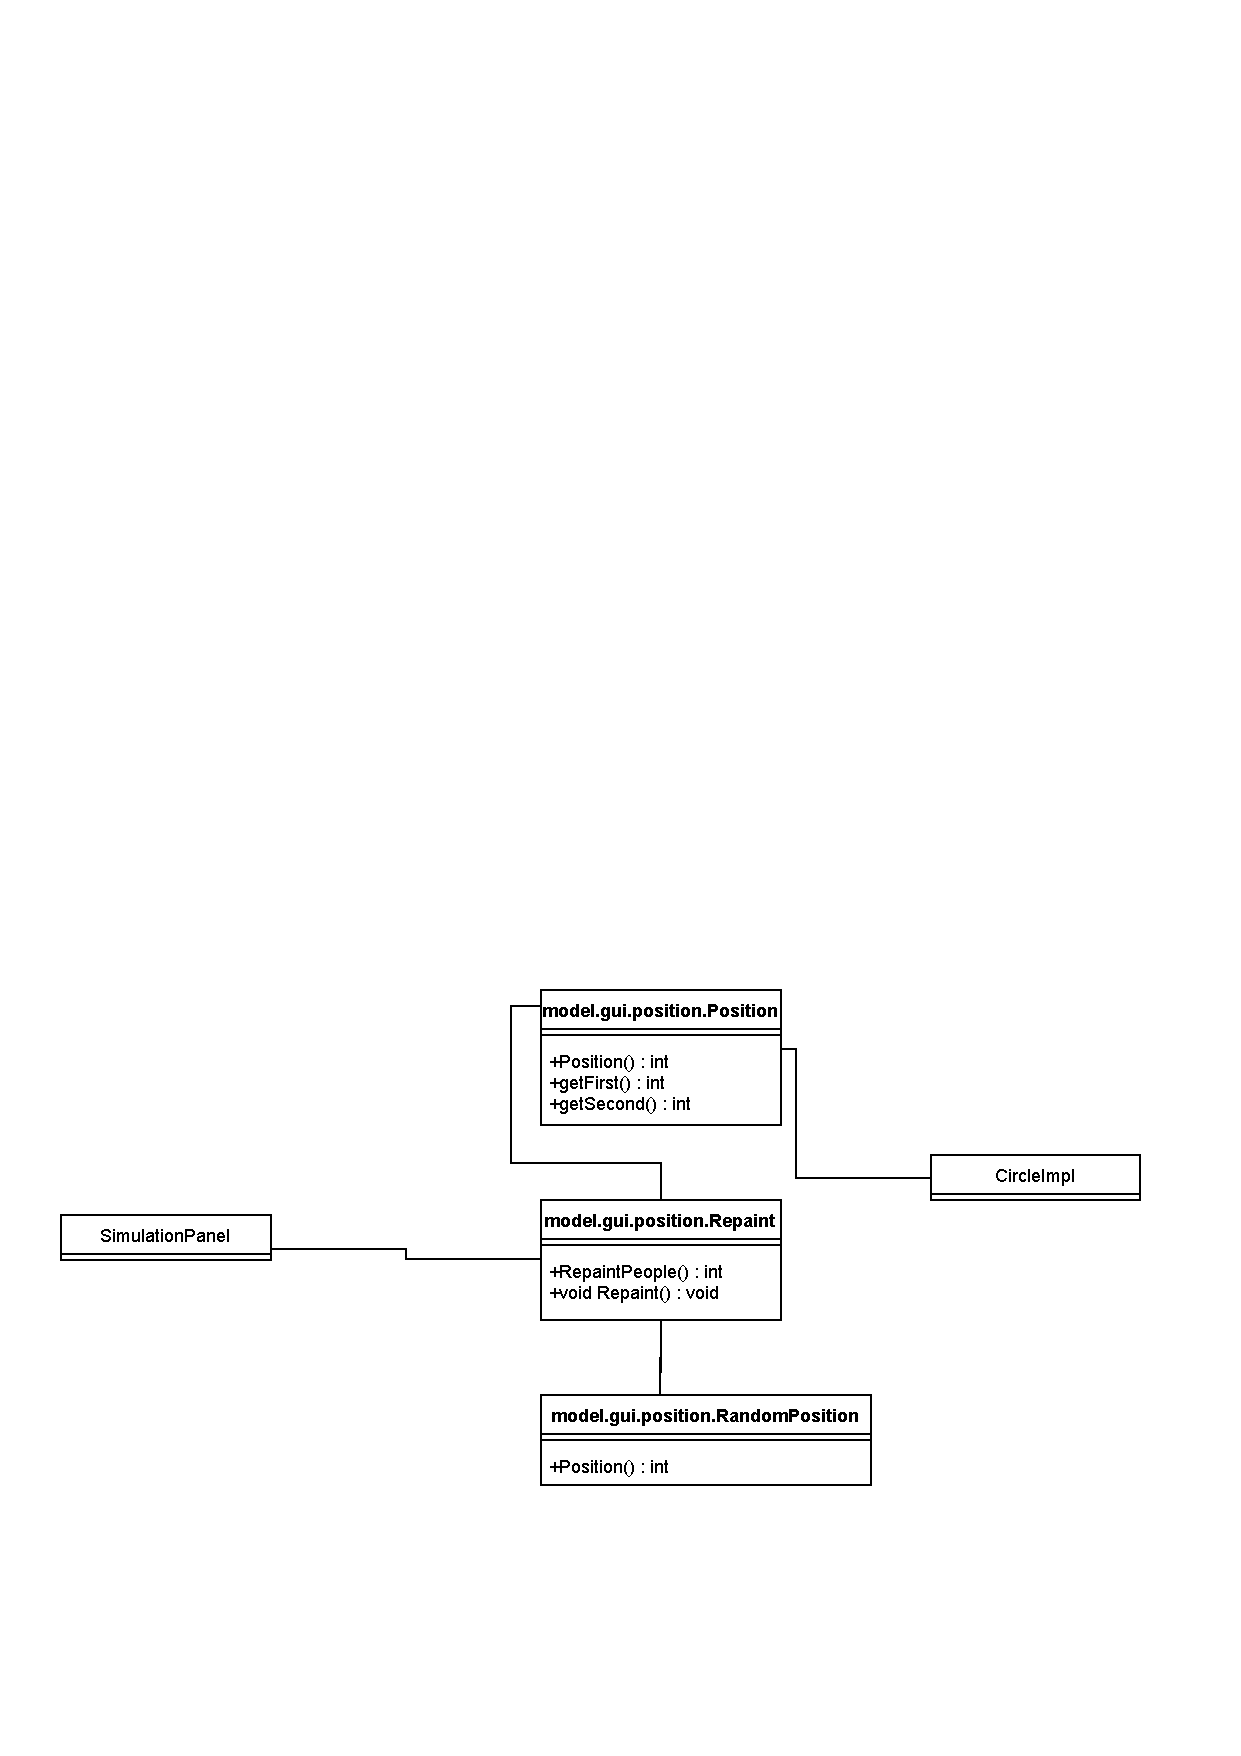
\includegraphics[width=.7\textwidth]{OOP-LiveLand/img/People_GUI_position.pdf}
\caption{Schema UML dell'aggiornamento della posizione delle persone nell'ambiente del parco.}
\label{img:People_GUI_position}
\end{figure}

\paragraph{Divisione in package:} Ho diviso le mie classi in quattro package principali. Per la suddivisione delle classi e delle interfacce nei package ho seguito una logica mettendo model.gui.person e model.gui.position, che si occupano di strutturare le persone e le loro posizioni, nel package gui. Il view.controller è il package in cui c’è l’interfaccia ViewController e la sua implementazione. View.gui ha all’interno la creazione del frame grafico e il design delle persone.\\\\\\\\\\


\paragraph{Livia Del Gaudio}
\paragraph{} I punti da me sviluppati nella realizzazione del progetto includono la creazione e l’inserimento delle attività all’interno dell’ambiente della simulazione, la produzione dell’analisi finale della simulazione ed il salvataggio di quest’ultima su file a scelta dell’utente o su un file di default. Ho cercato di rispondere a queste richieste implementando il più possibile il pattern MVC per ottenere un’adeguata separazione dei concetti.

\paragraph{Problema} Costruzione di una nuova attività
\paragraph{Soluzione} Per quanto riguarda la costruzione delle attività, che viene effettuata a run-time sulla base delle scelte dell’utente nelle finestre grafiche preposte (il cui comportamento è definito nell’interfaccia che entrambe implementano, ActivityGui), ho optato per la realizzazione della classe ViewActivity: essa funge da “ponte” tra View e Controller per passare i parametri inseriti dall’utente indipendentemente dal tipo di attività che si vuole istanziare. Questo è il motivo per cui al momento di creazione delle istanze di ViewActivity, implementato mediante il pattern creazionale Builder nella classe ViewActivityBuilder, è previsto che vi siano dei campi potenzialmente nulli (da qui deriva la scelta dell’uso di campi Optional), poiché a seconda del tipo di attività scelto essi saranno richiesti o meno. Infatti, per quanto riguarda le giostre, sia per adulti sia per bambini, è richiesto di inserire un nome, di scegliere il tipo di giostra e di inserire una capienza massima per ogni corsa. Per le attività redditizie invece, che includono sia negozi che ristoranti, è chiesto di impostare, oltre al nome e al tipo di attività, anche il range di prezzo pro capite per la suddetta attività. Inoltre, sia la classe ViewActivityImpl che ViewActivityBuilder fanno dunque uso del concetto di tipo di attività, incapsulato all’interno dell’enumerazione ActivityType, ove sono elencati i quattro tipi di attività previsti.

\begin{figure}[h]
\centering{}
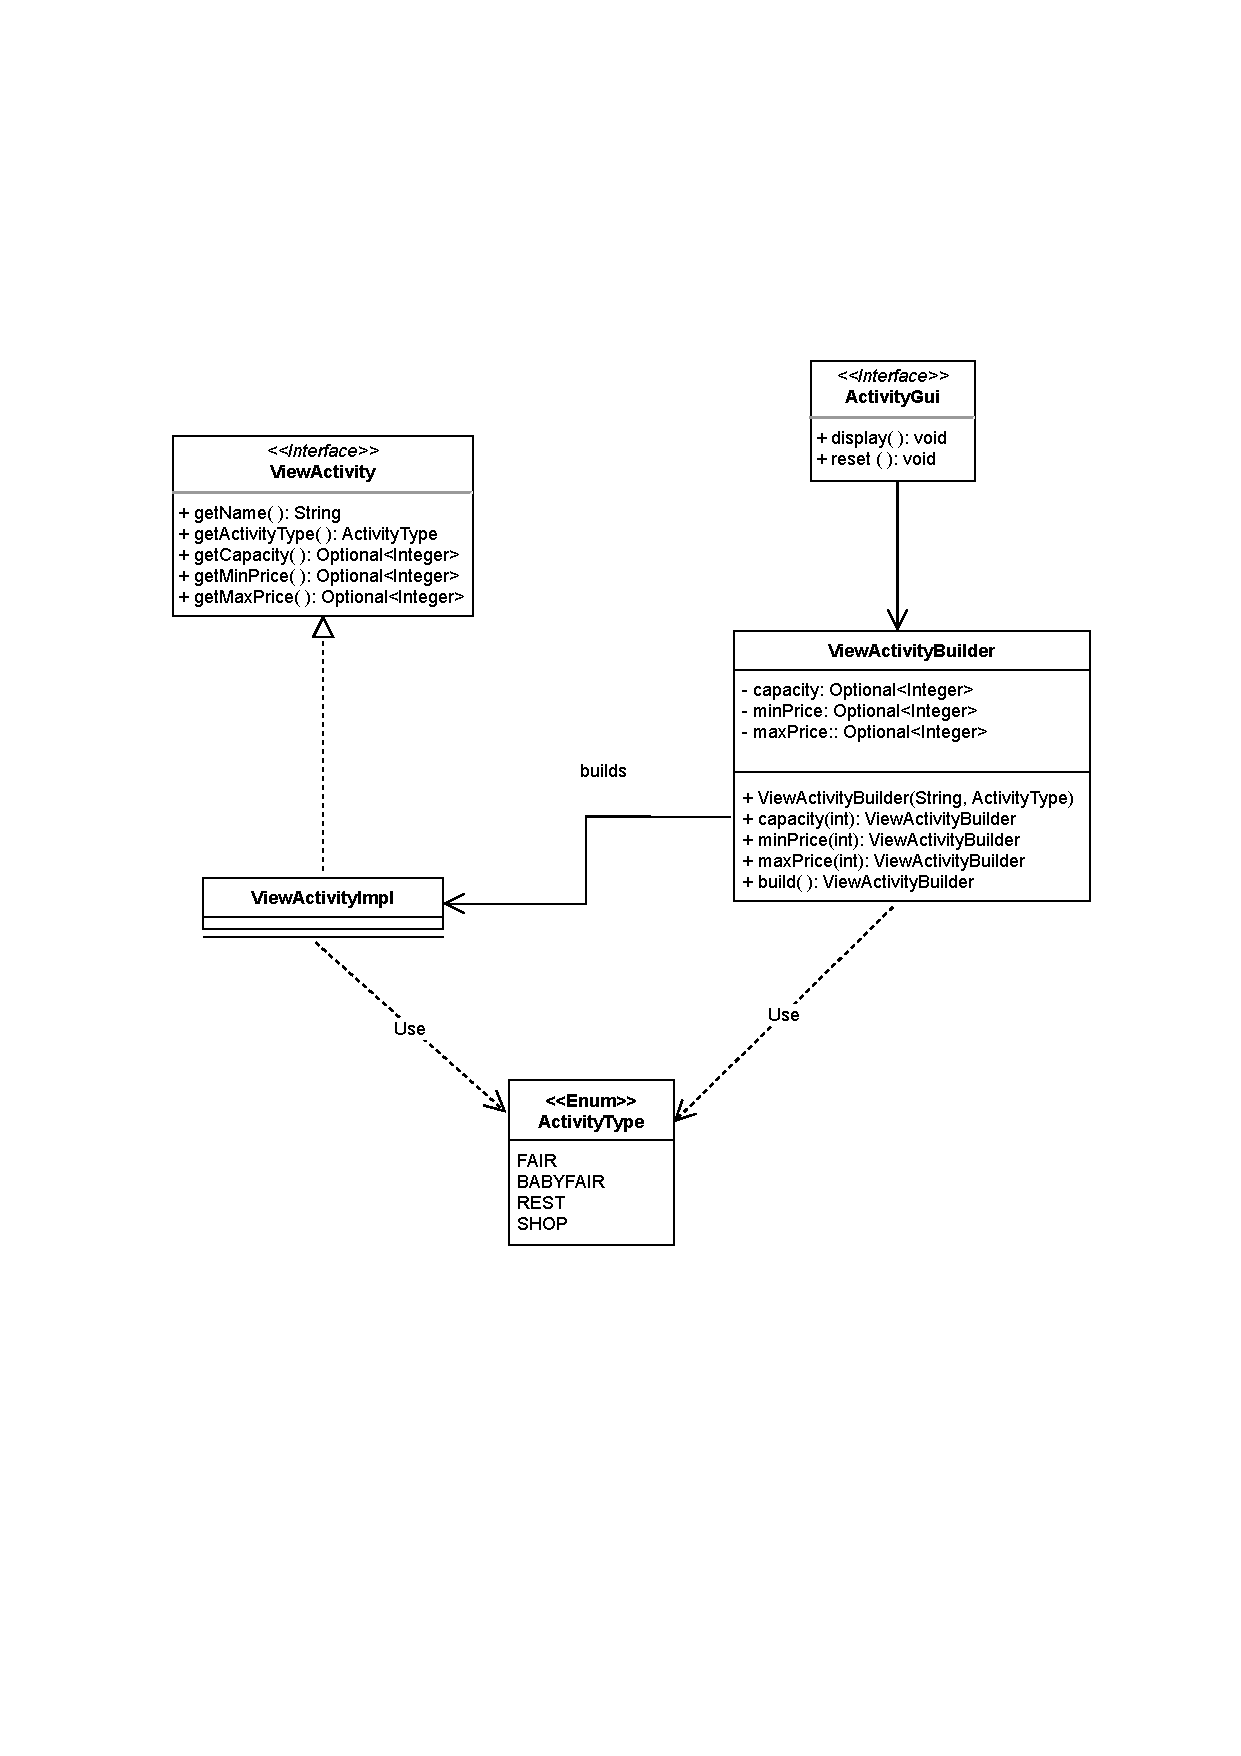
\includegraphics[width=.7\textwidth]{OOP-LiveLand/img/activity_building.pdf}
\caption{Schema UML della creazione di una nuova attività con i parametri inseriti dall'utente.}
\label{img:activity_building}
\end{figure}

\paragraph{\\\\Problema} inserimento di una nuova attività a scelta dell'utente.
\paragraph{Soluzione} Una volta che l’utente, dalla finestra del menu iniziale, decide di inserire una nuova attività e setta correttamente i parametri richiesti nella finestra ProfitGui o FairGui (a seconda del tipo scelto), viene creata la ViewActivity come precedentemente descritto, per poi passarla all’EnvironmentController che si occuperà di inserirla effettivamente all’interno della simulazione. Per fare ciò, il controller richiama il metodo apposito nell’ActivityEnvironment, ove sulla base del tipo di attività definito si istanziano effettivamente oggetti di tipo Fair e Profit con i valori scelti dall’utente. Il Model tiene poi traccia delle attività inserite in liste preposte, che sono accessibili al controller: esso dovrà infatti accedere alla rappresentazione interna del parco e notificarla alla finestra grafica della simulazione quando viene avviata.

\begin{figure}[h]
\centering{}
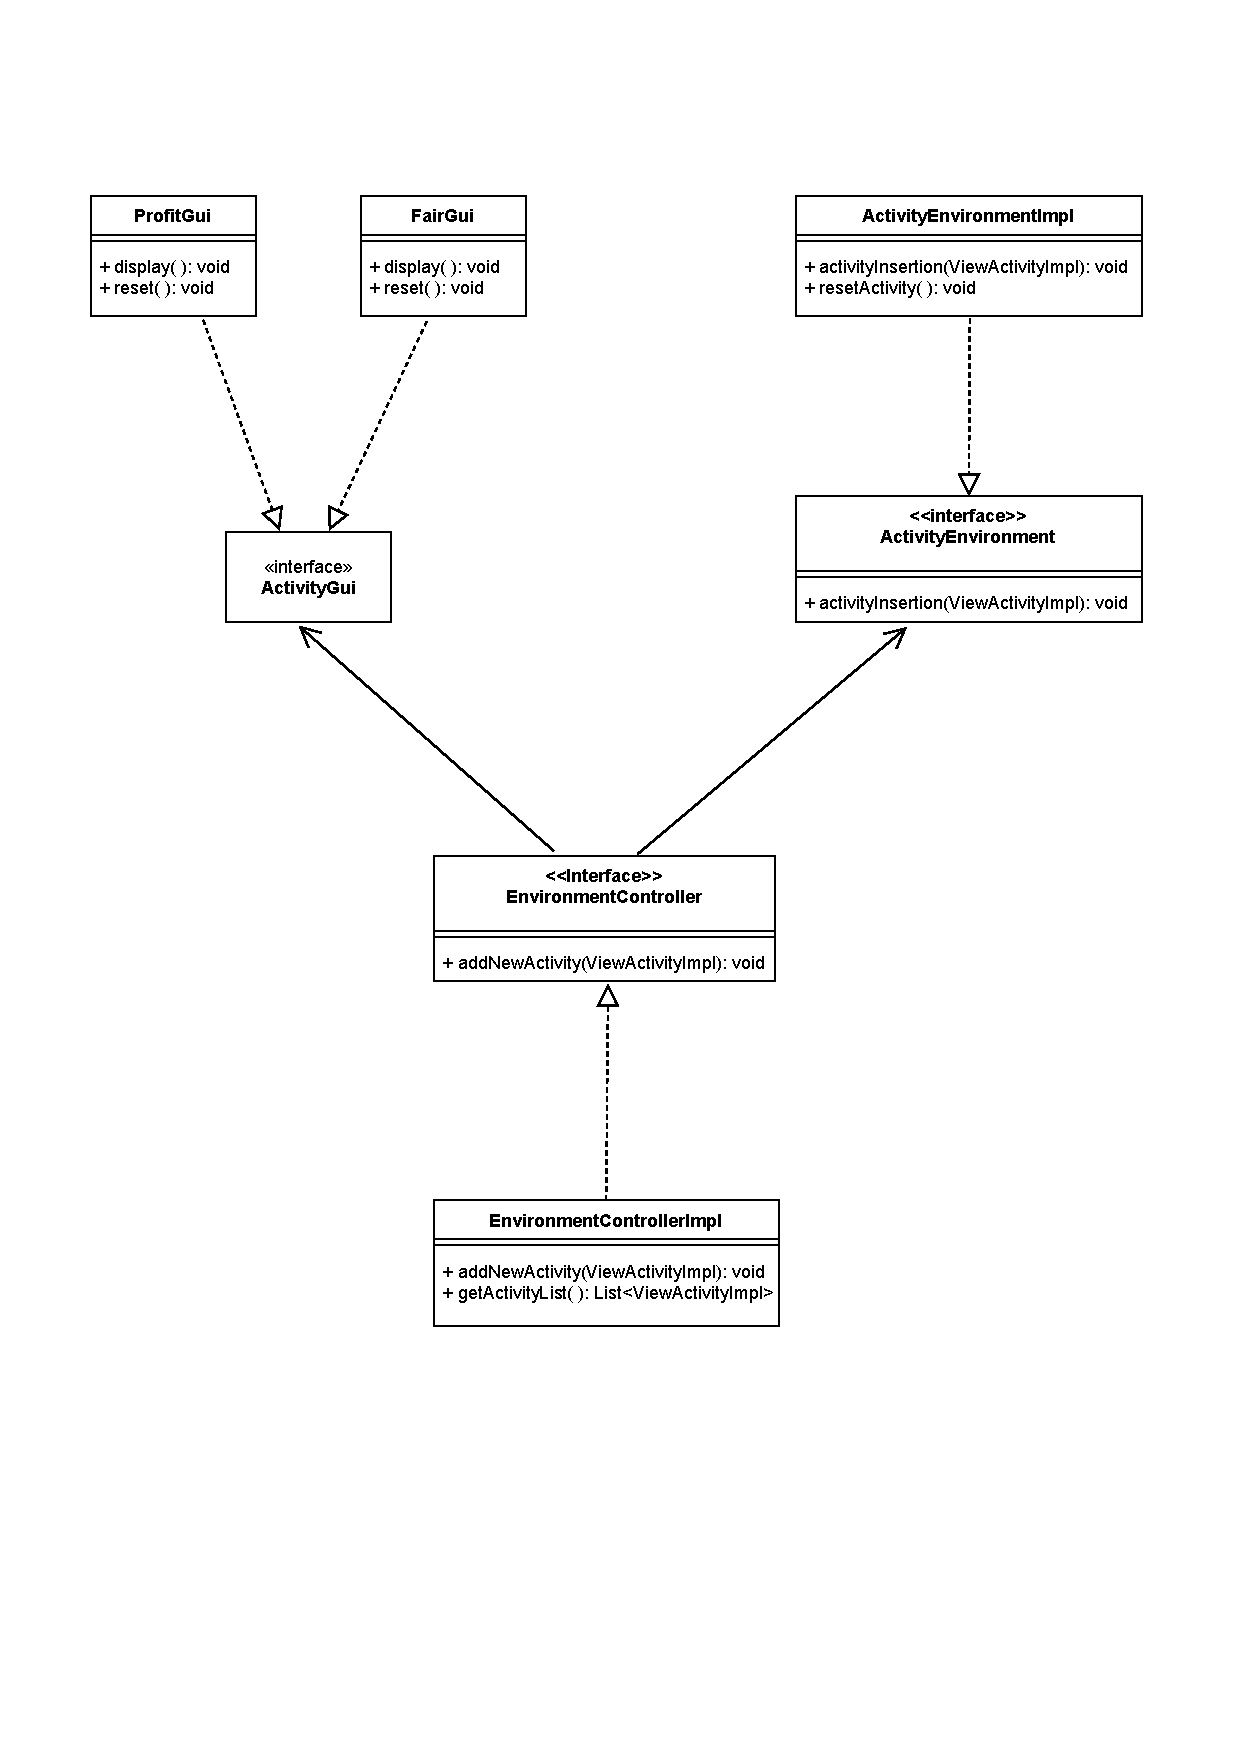
\includegraphics[width=.7\textwidth]{OOP-LiveLand/img/activity_insertion.pdf}
\caption{Schema UML dell'inserimento nell'environment del parco di una nuova attività.}
\label{img:activity_insertion}
\end{figure}

\paragraph{Problema} Produzione dell'analisi finale basata sui dati raccolti durante la simulazione
\paragraph{Soluzione} Al termine della simulazione viene predisposta una finestra grafica che mostra ciò che si è verificato all’interno del parco: al fine di ottenere una resa visiva maggiore, ho optato per la produzione di grafici e statistiche che mostrassero i dati raccolti. Per fare ciò mi sono servita delle librerie esterne di JFreeChart, creando due grafici diversi sulla base del focus da rappresentare: nel caso del gradimento delle giostre ho optato per un grafico a torta, mentre per gli incassi giornalieri ho utilizzato un grafico a barre. La logica di produzione dell’analisi era simile per entrambe le statistiche, ma l’implementazione interna differiva: ho dunque deciso di costruire le due rappresentazioni seguendo il pattern AbstractFactory estendendo una classe astratta in cui sono dichiarati i metodi per l’inserimento dei dati acquisiti in un dataset, sulla base del quale viene generato il grafico. Queste classi, rappresentanti il Model per la produzione dell’analisi, sono interrogate da un apposito controller, AnalysisController, che notifica alla View. Essa è costituita dalla finestra grafica AnalysisDialog, la quale si apre una volta che l’utente stoppa la simulazione, con l’intento di mostrare i grafici creati.

\begin{figure}[h]
\centering{}
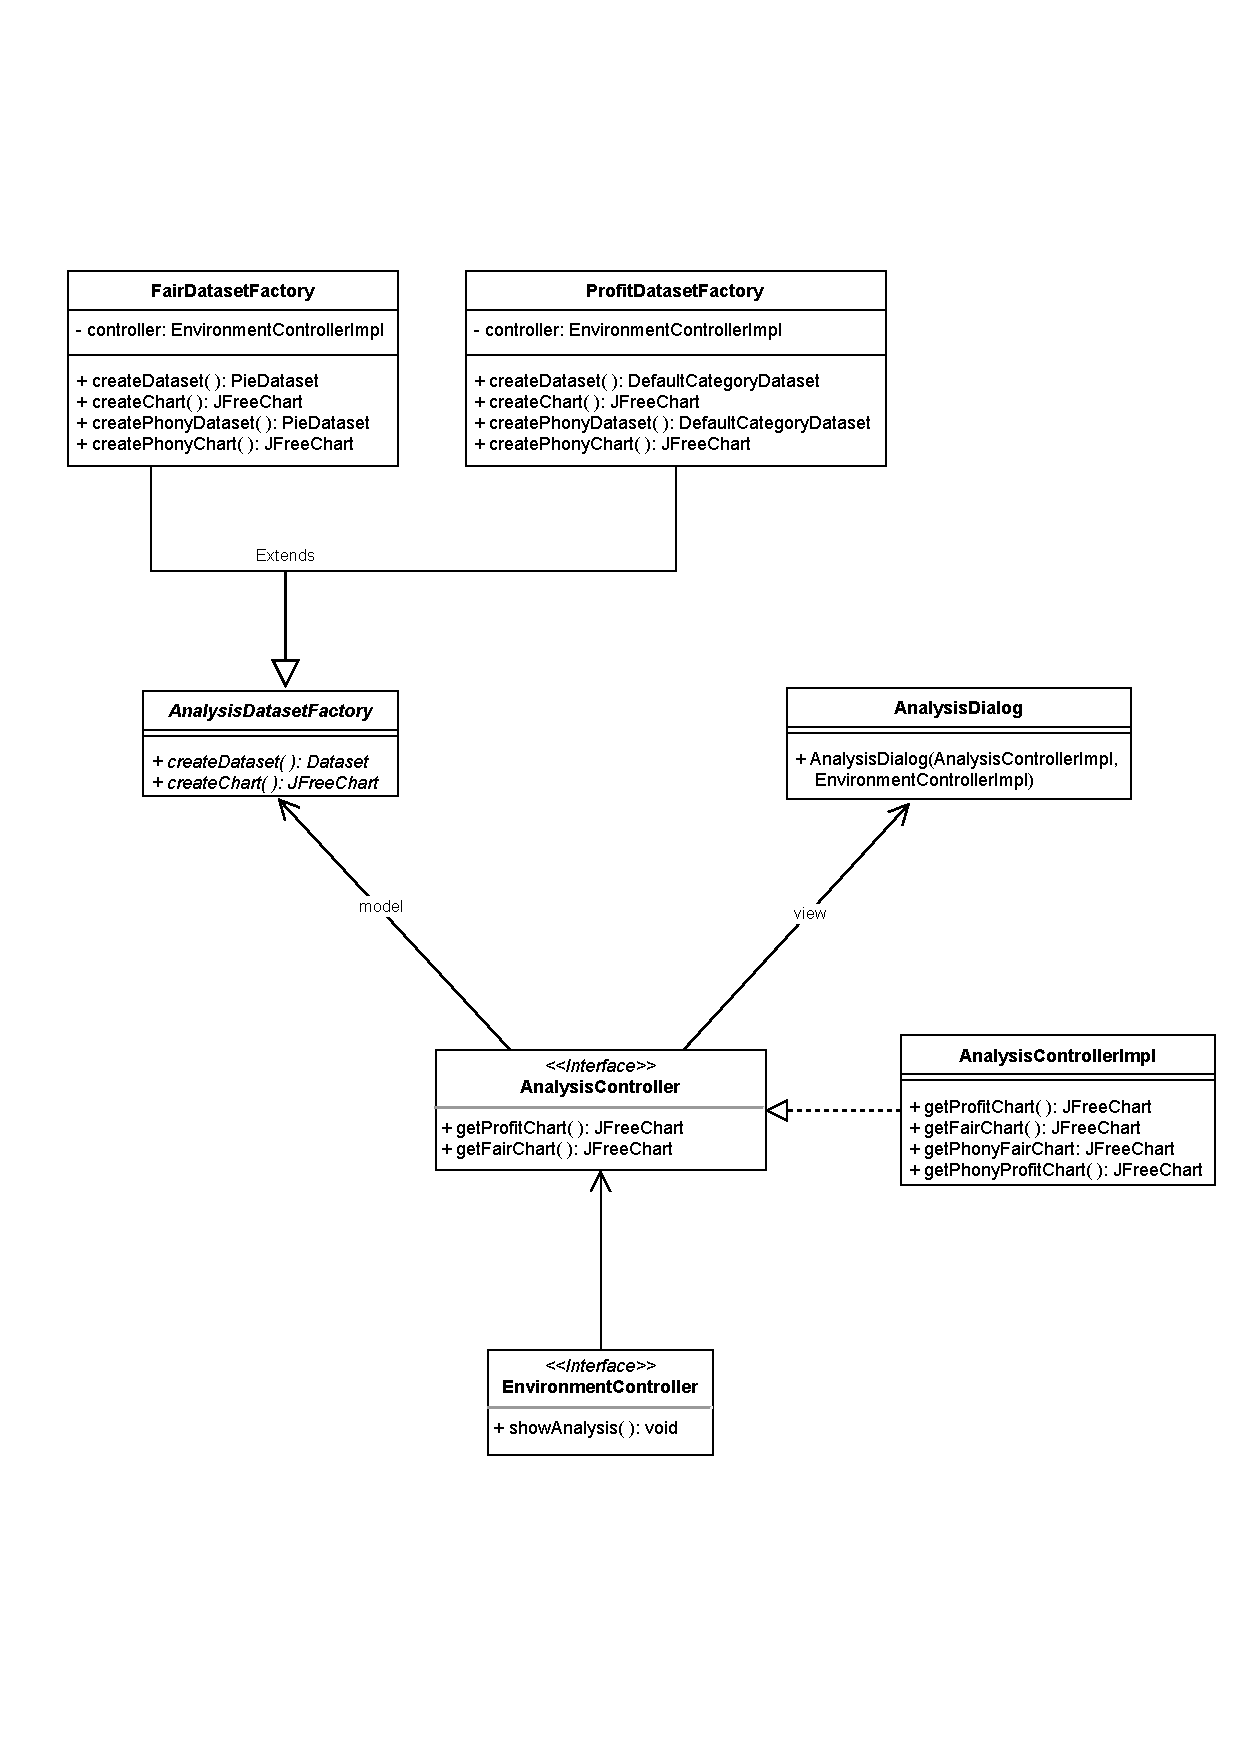
\includegraphics[width=.7\textwidth]{OOP-LiveLand/img/analysis_factory.pdf}
\caption{Schema UML della produzione dell'analisi finale sulla base dei dati raccolti nella simulazione.}
\label{img:analysis_factory}
\end{figure}

\paragraph{Problema} salvataggio dell'analisi generata su un file a scelta dell'utente.
\paragraph{Soluzione} All’interno dell’AnalysisDialog viene mostrato il SaveAnalysisMenu, un JMenu che ha il compito di coordinare il salvataggio su file dell’analisi prodotta. A seconda della scelta dell’utente nel menu di salvataggio, viene richiesto al controller di impostare la destinazione, qualora l’utente lo desideri (altrimenti il file di default è ~/output.txt) e successivamente di salvare la rappresentazione dell’analisi. Ho risposto a questo problema mediante l’utilizzo di un PrintStream, sulla scorta di quanto visto in laboratorio durante il corso. La rappresentazione testuale dell’analisi viene prodotta dalla classe AnalysisImpl, che costituisce il Model di questa sotto-parte: dal momento che ho lavorato con gli Stream per il salvataggio, mi è stato necessario stampare sul file scelto solo una concatenzione di stringhe di testo che descrivono i dati raccolti nella simulazione. Tuttavia, la mia idea iniziale era quella di salvare sul file entrambe le statistiche prodotte come immagini, ma di fatto l’immagine non veniva aggiunta come avrei voluto. Di conseguenza, ho previsto una terza opzione nel JMenu, avvalendomi del metodo fornito da JFreeChart per salvare le statistiche ottenute sotto forma di file jpeg, dando dunque all’utente la possibilità di salvarle nella propria home directory con nomi predefiniti. Per realizzare quest’ultima feature ho creato una classe apposita, ChartImgBuilder e la relativa interfaccia.

\begin{figure}[h]
\centering{}
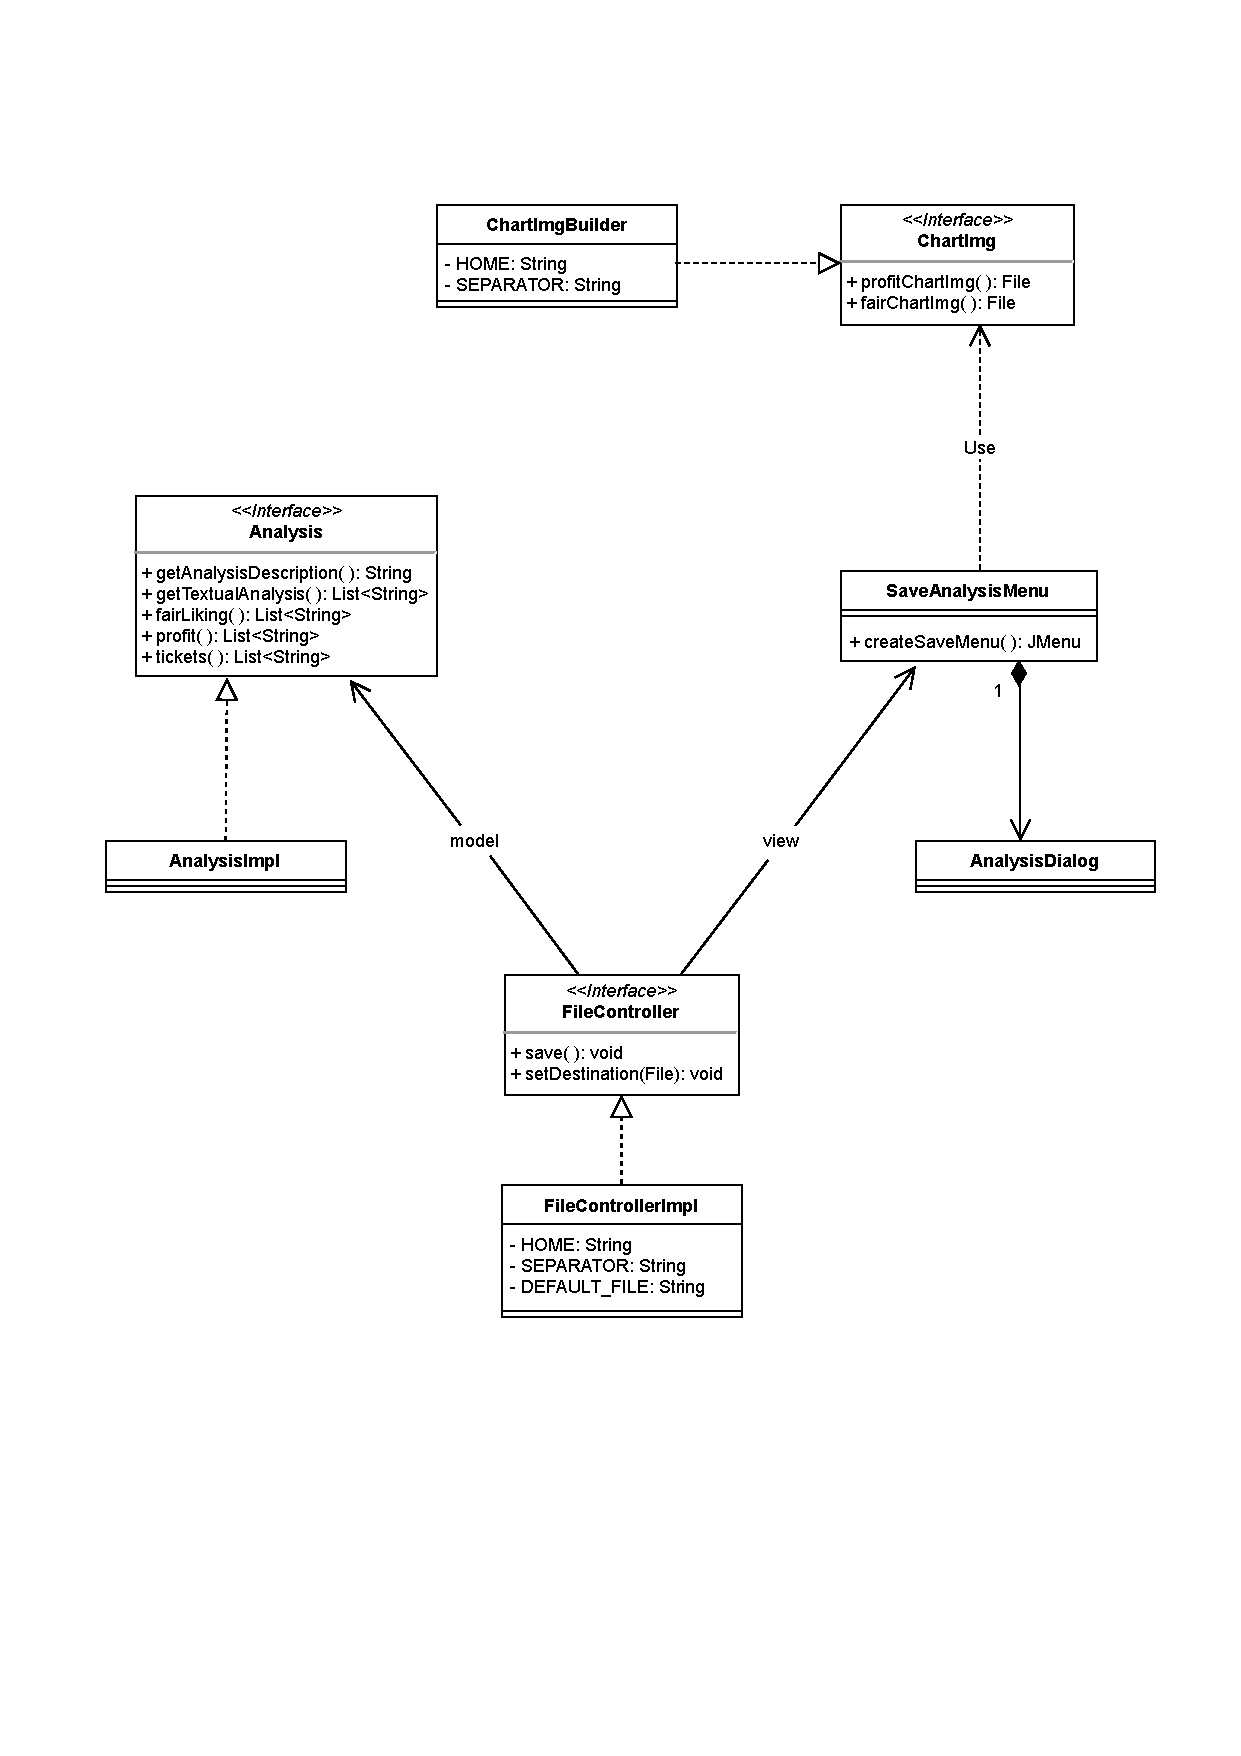
\includegraphics[width=.6\textwidth]{OOP-LiveLand/img/analysis_saving.pdf}
\caption{Schema UML del salvataggio dell'analisi prodotta su file.}
\label{img:analysis_saving}
\end{figure}

\paragraph{Divisione in package:}
Per quanto riguarda il Model, ho suddiviso i miei package sulla base del problema cui rispondono: model.environment.activity si occupa dell’inserimento delle attività all’interno del parco, model.environment.visitors si occupa di impostare la capienza massima del parco (richiesta all’inizio della simulazione dalla View e opportunamente passata all’EnvironmentController), model.analysis della produzione dei Dataset e dei grafici e model.analysis.save cura la rappresentazione testuale dell’analisi generata e il salvataggio dei grafici in formato jpeg.
Per quanto riguarda la sezione Controller invece, ho creato il package controller in cui, oltre alle classi già spiegate e mostrate in precedenza con UML, è presente anche il Controller principale che viene creato nel main e ha il compito di settare la View del menu e l’EnvironmentController. Quest’ultimo si occupa inoltre di far partire e chiudere la simulazione, mostrando le finestre grafiche opportune e facendo partire al momento di avvio effettivo della simulazione il Thread principale mediante la classe Simulator, che estende Runnable. A questa feature abbiamo lavorato insieme io e Ines Fraccalvieri.
Riguardo la View, sono presenti tre package che gestiscono le tre possibili finestre grafiche del menu: quella principale, la GraphicalUserInterface, che richiama quando richiesto dall’utente le altre due, ovvero ProfitGui e FairGui. Esse sono contenute rispettivamente nei package view.menu, view.menu.fair e view.menu.profit, ove sono presenti, oltre ai pannelli utilizzati, anche le eccezioni previste qualora l’utente tentasse di avviare la simulazione senza aver inserito adeguatamente i valori richiesti. 
Infine, è presente un package “ibrido” tra View e Model che si occupa della creazione momentanea di un oggetto in cui vengono salvati i campi inseriti dall’utente nella View per rendere il passaggio al Controller e al Model più semplice ed efficiente. Per questo motivo il package che si occupa di questa feature è stato chiamato view.model.activity.

\onecolumn
\paragraph{Ines Fraccalvieri}

\paragraph{Problema} Inserimento delle persone all'interno del parco, che per accedervi devono essere associate a un biglietto.
\paragraph{Soluzione} La classe PersonTicket rappresenta le persone che sono all'interno del parco. All'interno possiamo trovare due metodi principali randAge() e randTicket().
Il primo genera un numero random tra un AGEMIN e un AGEMAX, che indica l'età massima e minima che può essere generata e associata ad una persona.
randTicket() invece, in modo random associa un biglietto giornaliero (facendo un controllo per vedere a quale fascia di età appartiene, se è maggiore di 65 o minore di 12 otterrà il biglietto REDUCED altrimenti sarà ADULT) o un abbonamento SEASONPASS.

\begin{figure}[h]
\centering{}
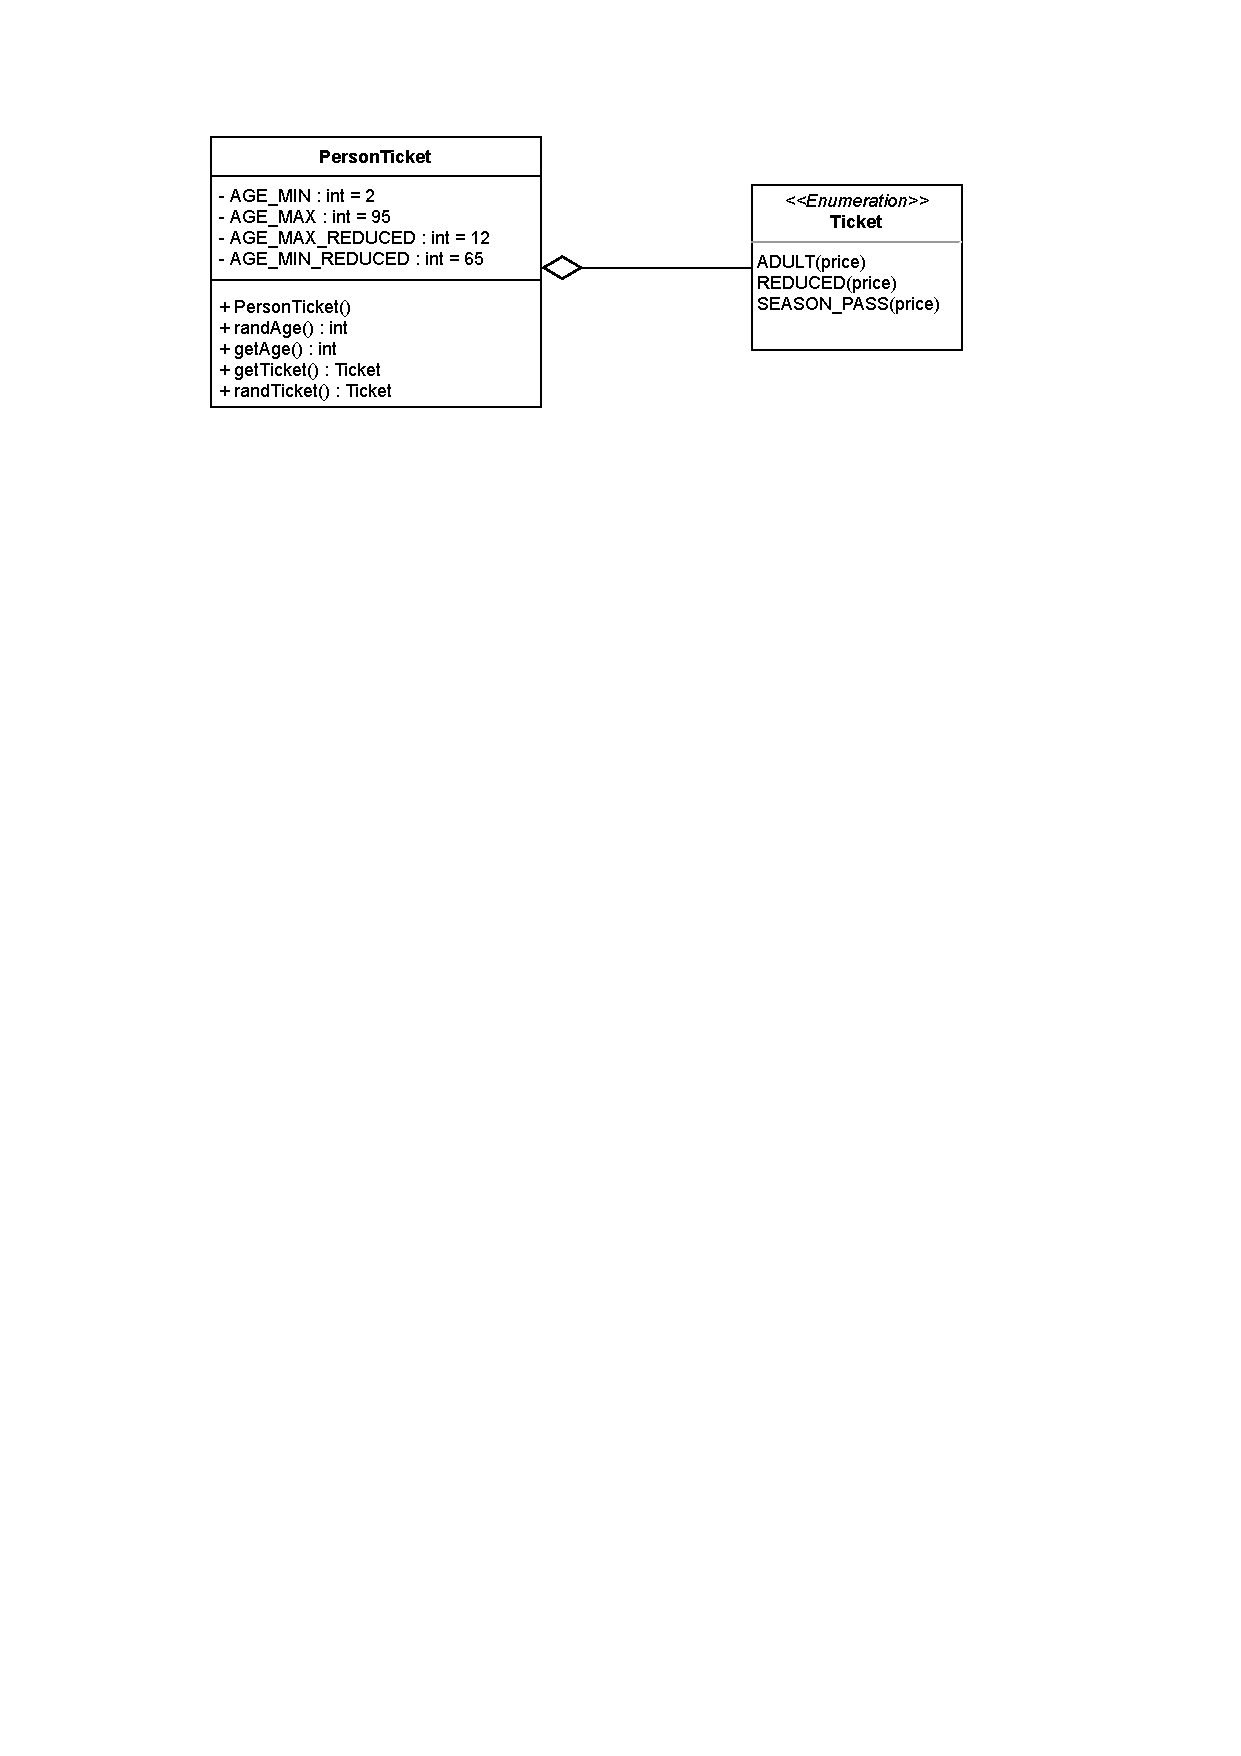
\includegraphics[width=.7\textwidth]{OOP-LiveLand/img/Person-Ticket.pdf}
\caption{Schema UML della creazione di persoe cui è associato un biglietto.}
\label{img:Person-Ticket}
\end{figure}

\paragraph{Problema} Gestione delle entrate e delle uscite delle persone all'interno del parco
\paragraph{Soluzione} La gestione dell'entrata e dell'uscita delle persone all'interno del parco è organizzata dall'EnvironmentImpl, che implementa l'interfaccia Environment. Alla partenza della simulazione, grazie alla classe OpenImpl, vengono generati un numero  random di persone che entrano subito nel parco.
Tutte le persone accedono al parco attraverso l'EnvironmentImpl, responsabile di inserirle all'interno di una lista personList, che tiene traccia delle persone che sono all'interno del parco ma non stanno facendo nessuna attività in esso presente.
Quando si accede al parco si passa da EntranceImpl, la biglietteria del parco, che tiene il conteggio del profitto, suddiviso in tipo di biglietto ai fini di una buona analisi finale, per osservare quale tipologia è la più venduta.

\begin{figure}[h]
\centering{}
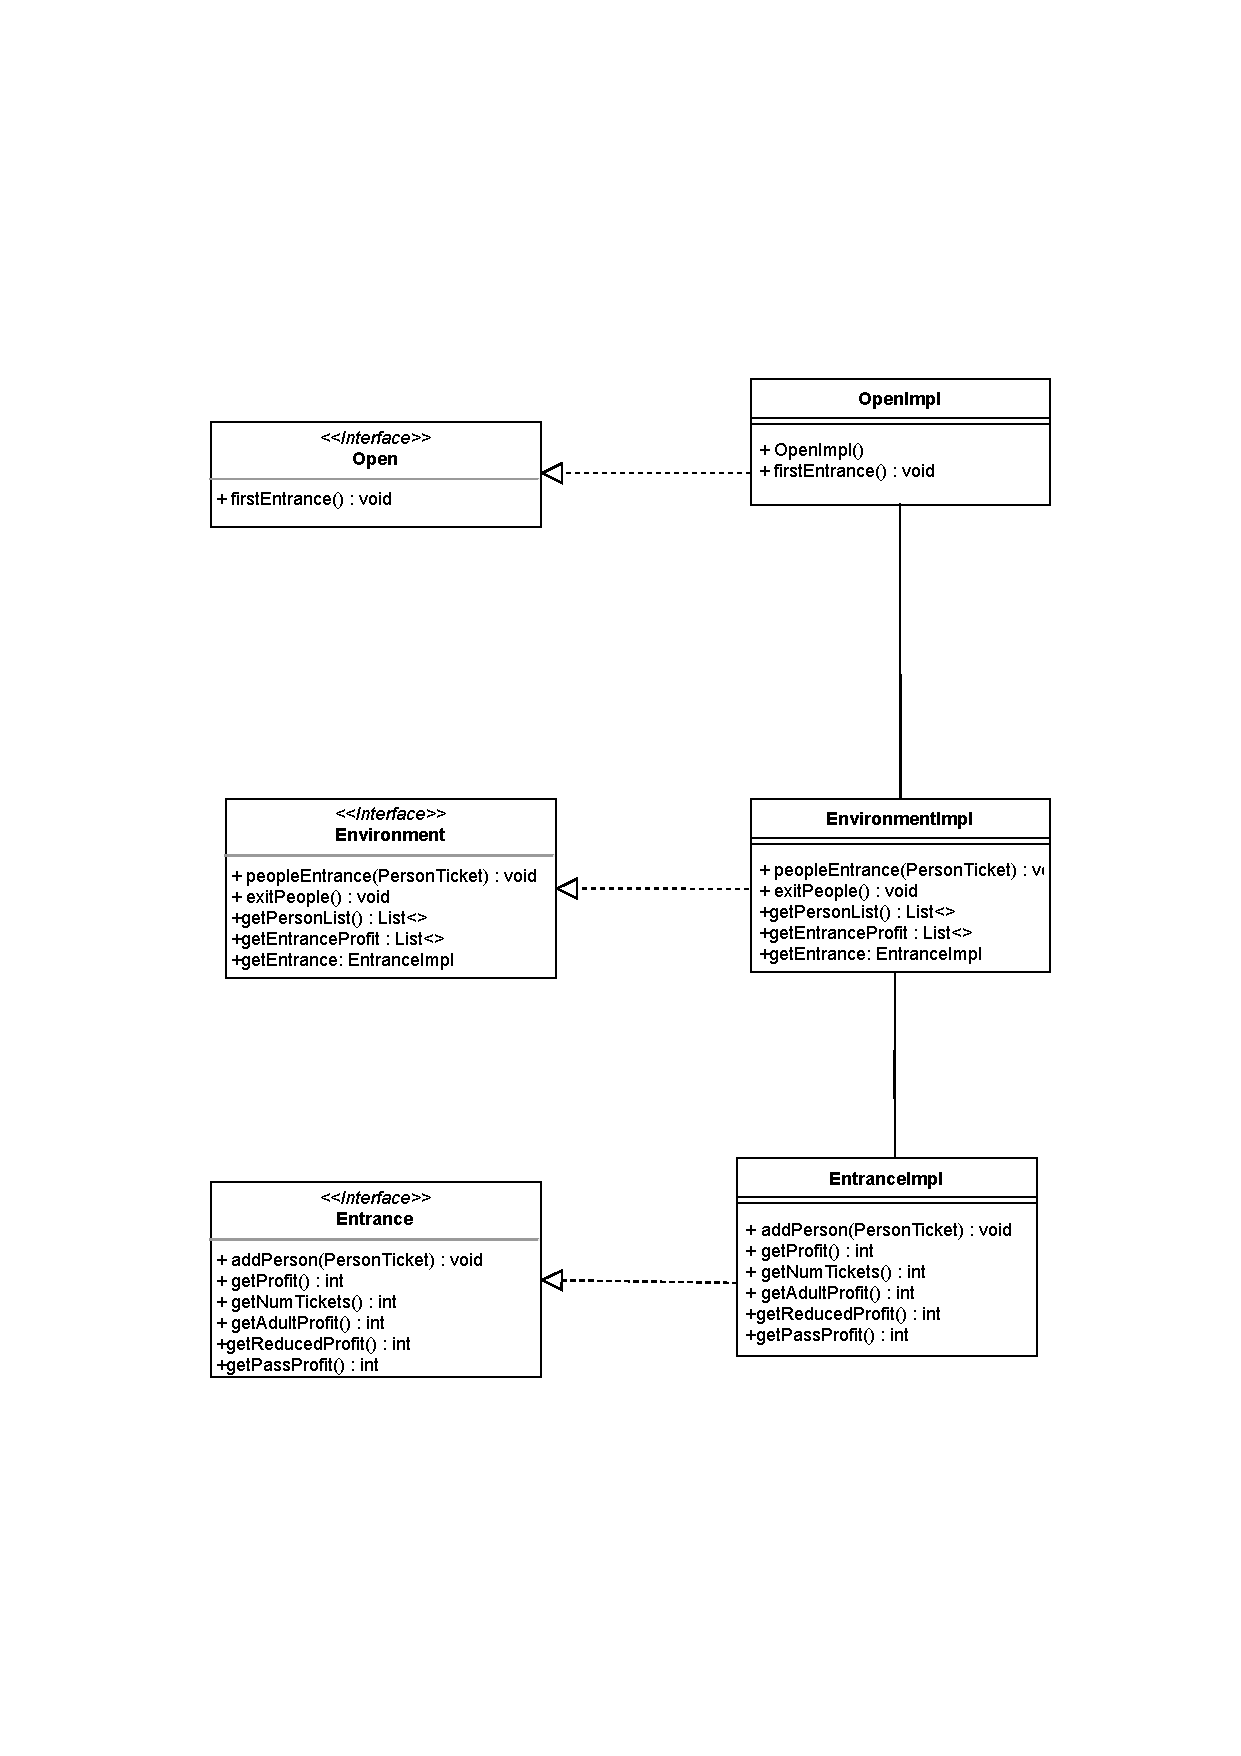
\includegraphics[width=.7\textwidth]{OOP-LiveLand/img/People_Entrance.pdf}
\caption{Schema UML della gestione dell'entrata delle persone all'interno del parco.}
\label{img:People_Entrance}
\end{figure}

\paragraph{Problema} Gestione del movimento interno al parco dal punto di vista logico delle persone
\paragraph{Soluzione} La gestione del movimento logico delle persone all'interno del parco è coordinata da PersonIntoPark, PeopleRecirculation e ActivityRide.
La classe PersonIntoPark estende un Thread che gestisce il richiamo di quest'ultime.
Nel metodo run() fa partire la simulazione richiamando OpenImpl, che come precedentemente citato, che inserisce un numero random di persone all'apertura del parco.
Mentre il metodo logics() coordina l'entrata e l'uscita di esse in modo casuale nel parco, invocando la classe PeopleRecirculation.
Al suo interno troviamo il metodo principale recirculation(), che accedendo alla lista delle persone presenti e alla capienza massima del parco, genera numeri casuali per poter evitare di creare un eccezione 
e far si che il totale non sia mai negativo o che non supero il numero di visitatori scelto dall'utente.
L'ultima classe che viene richiamata da PersonIntoPark è ActivityRide.
Quest'ultima simula la corsa delle attività presenti nel parco. Per ognuna di esse viene estratto un valore random, che sarà associato al numero di persone che potranno accedervi. Per le giostre viene fatto un ulteriore controllo in modo che non 
ecceda mai la sua capacità, anch'essa determinata a discrezione dell'utente.

\begin{figure}[h]
\centering{}
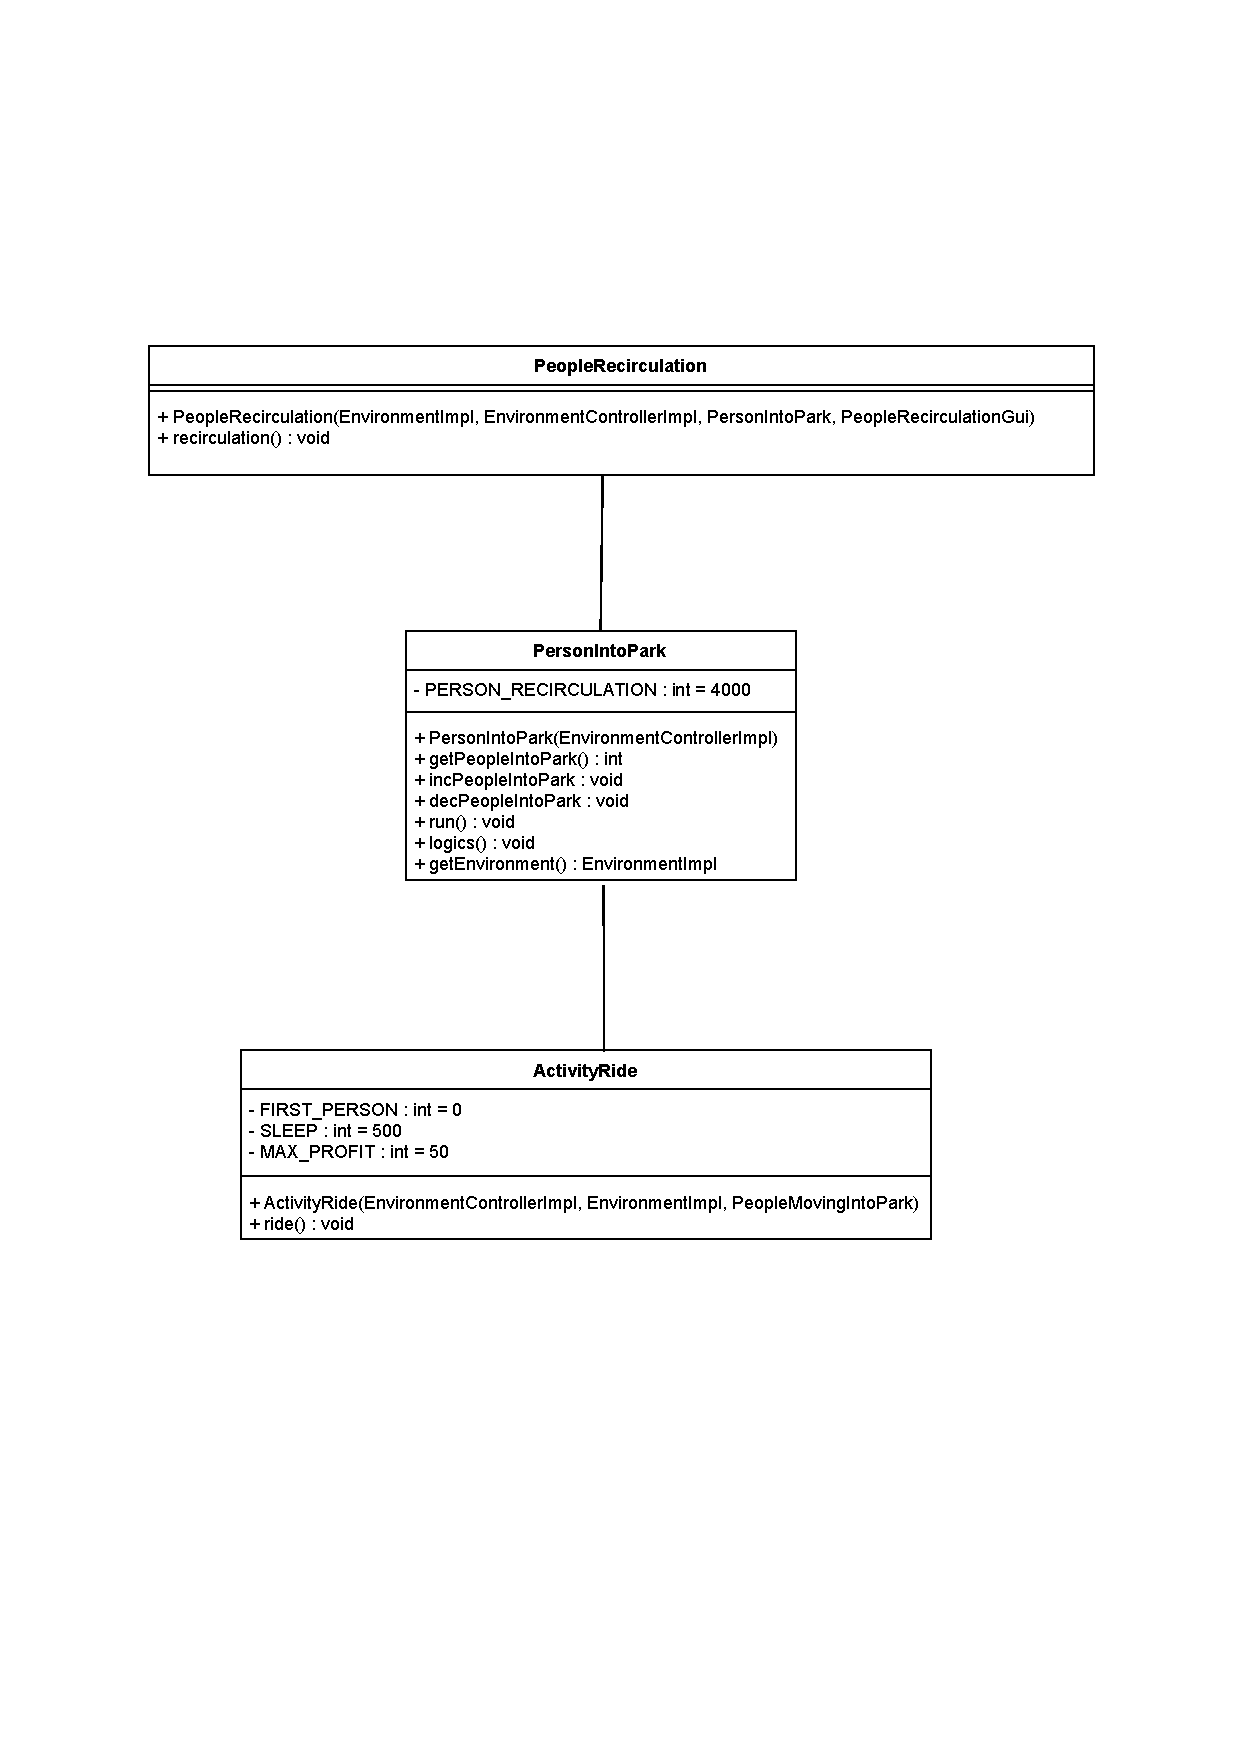
\includegraphics[width=.6\textwidth]{OOP-LiveLand/img/People_moving_into_park.pdf}
\caption{Schema UML della gestione del movimento delle perone all'interno del parco.}
\label{img:People_Moving}
\end{figure}

\paragraph{Divisione in package:} Ho scelto di operare una suddivisione in package tale da raggruppare le classi e interfacce correlate tra di loro in un unico package. I package principali che gestiscono la creazione sono model.ticket e model.person.ticket. Nel primo troviamo un Enum della tipologia del biglietti con associato il rispettivo prezzo, nel secondo, invece, vengono connesse le persone al ticket, facendo controlli sull’età per assicurarsi che vengano rispettate le condizioni per l’acquisto del biglietto.
Inoltre possiamo trovare due ulteriori package che coordinano l’ingresso delle persone, model.person.environment, che gestisce l’entrata fisica di esse, mentre model.person.entrance tiene traccia del profitto ricavato dalla vendita dei biglietti con il fine di creare una buona analisi finale dell’andamento del parco.
Infine ho creato un ultimo package, people.environment.controller, che raggruppa le classi utilizzate per il movimento logico delle persone, entrata, uscita e l’accesso alle attività, mantenendo sempre il numero totale al di sotto delle varie capienze fornite dall’utente.

\chapter{Sviluppo}
\section{Testing automatizzato}

Il testing automatizzato  per questo progetto è stato effettuato attraverso la suite JUnit5. Viste le numerose componenti grafiche presenti nell'applicazione e l'interazione richiesta all'utente in fase iniziale per la costruzione dell'ambiente interno del parco, si è deciso di testare le seguenti componenti:


\begin{itemize}
 \item ActivityFairTest: Testa la creazione di una attività fair.
 \item ActivityProfitTest: Testa la creazione di una attività profit.
 \item ActivityInsertionTest: Testa la corretta creazione di oggetti ViewActivityImpl, il relativo inserimento all'interno della simulazione mediante l'intervento dell'EnvironmentController ed infine il reset delle attività precedentemente aggiunte.
 \item PersonAndParkTest: Testa la corretta apertura del parco, facendo entrare un numero random di persone, per poi farle uscire. Inoltre verifica che si tenga traccia coerentemente degli incassi derivanti dalla vendita dei biglietti associati alle persone che entrano.
 \item AnalysisDatasetTest: Testa, sulla base di metodi appositi aggiunti per creare statistiche "fasulle" predefinite, la corretta generazione dei dataset riguardanti il gradimento delle giostre e gli incassi giornalieri, per poi crearne i relativi grafici.
 \item TextualAnalysisTest: Testa il salavataggio su file di PhonyAnalysisImpl, un'analisi testuale predefinita.
\end{itemize}

Per quanto riguarda la parte grafica invece, si è preferito testare manualmente i componenti, per verificarne il corretto funzionamento e che fornisse effettivamente la resa grafica desiderata. Per facilitare questa operazione, si è optato per l'inserimento di un pulsante che velocizzasse il setting iniziale degli ambienti, prevedendo una configurazione di default.

\section{Metodologia di lavoro}

La fase di progettazione e design iniziale è stata svolta interamente insieme, cercando di convenire sulle interfacce da utilizzare in ciascuna sottoparte, per rendere la programmazione successiva più agile e strutturata. Tuttavia, durante la fase successiva ci siamo accorte in più occasioni che il design iniziale non era del tutto efficiente e che era difficile da sviluppare dal punto di vista implementativo, oppure semplicemente abbiamo trovato modi più performanti per risolvere determinati problemi.
La ripartizione del lavoro individuale è stata la seguente:

\begin{itemize}
	\item Casadei Valentina: implementazione delle attività presenti nella simulazione, relativa rappresentazione grafica nel pannello della simulazione e definizione randomizzata della spesa di ogni persona per le attviità redditizie, necessaria ai fini dell'analisi finale.
	\item Contrini Enrica: gestione dello spostamento a livello grafico delle persone, distinte sulla base dell'età e della tipologia di biglietto cui vengono associate all'ingresso, implementando il pattern MVC.
	\item Del Gaudio Livia: gestione del menu iniziale e della disposizione interna delle attività sulla base delle scelte dell'utente, produzione dell'analisi finale e possibilità di salvataggio su un file arbitrario.
	\item Fraccalvieri Ines: creazione delle persone, associazione ai vari tipi di biglietto tenendo traccia degli incassi ottenuti, gestione entrate e uscite delle persone a livello logico e relativo movimento verso le attività presenti.
\end{itemize}

Dopo aver lavorato in modo individuale cercando di rispondere agli obiettivi principali prefissati, ci siamo trovate a lavorare in coppie per cercare di unire il lavoro svolto: Fraccalvieri e Del Gaudio hanno lavorato per cercare di far partire il thread principale PersonIntoPark dall'EnvironmentController, mentre Contrini e Casadei hanno lavorato all'interfaccia grafica, aggiungendo le attività create nel pannello della simulazione e gestendo il repaint delle persone ad ogni ciclo del thread principale. Infine ci siamo trovate per integrare tutti i componenenti del progetto e testarne il funzionamento finale, risolvendo eventuali problemi sorti.

\paragraph{}Per quanto riguarda la gestione del repository, abbiamo adottato il seguente workflow:

\begin{itemize}
	\item Ciascun membro del gruppo ha lavorato alle proprie features su branch appositi.
	\item Il branch develop è stato impiegato per fare merge delle features una volta portate a termine, e per risolvere eventuali conflitti e malfunzionamenti una volta effettuati i merge.
	\item Il branch master è stato impiegato unicamente per pushare la versione finale dell'applicazione.
	\item Quando abbiamo iniziato a lavorare agli ultimi dettagli in coppie, ci siamo spostate su branch dedicati all'integrazione del codice.
\end{itemize}

\section{Note di sviluppo}

\paragraph{Valentina Casadei}
\begin{itemize}
\item \textbf{JUnit5:} libreria utilizzata per il testing. automatizzato.
\item \textbf{Spunti presi da internet:} utilizzati per la rappresentazione grafica delle attività.
\end{itemize}

\paragraph{Enrica Contrini}
\begin{itemize}
\item \textbf{Spunti presi da fonti esterne:} per quanto riguarda l'impostazione della finestra grafica principale, per capire come strutturare il lavoro mi sono ispirata all'appliacazione BacteriaSimulator, designato su Virtuale come progetto ben fatto.
\end{itemize}

\paragraph{Livia Del Gaudio}
\begin{itemize}
\item \textbf{Stream e lambda:} impiegati ove possibile per action listeners e per cicli, in particolare per il controllo sulle attività già presenti nella simulazione.
\item \textbf{OutputStream:} declinato nella forma PrintStream per il salvataggio su file dell'analisi finale. 
\item \textbf{Optional:} impiegato al momento di building delle istanze di ViewActivityImpl.
\item \textbf{Concorrenza:} congiuntamente con Ines Fraccalvieri per garantire il corretto funzionamento interno del parco.
\item \textbf{Utilizzo della libreria JFreeChart:} per la creazione dei grafici al termine della simulazione. Ho cercato esempi di utilizzo su internet per capirne il funzionamento e riadattarlo alle mie esigenze.
\end{itemize}

Inoltre, ho cercato di seguire in maniera pervasiva quanto ci è stato mostrato a lezione, basandomi molto sui codici che ci hanno fornito per prenderne spunto (in particolare per quanto riguarda l’aspetto grafico e l’implementazione dei pattern). Per realizzare il JMenu necessario per scegliere come salvare l'analisi ho cercato su internet esempi della sua implementazione e li ho modificati per adattarli al funzionamento desiderato.

\paragraph{Ines Fraccalvieri}
\begin{itemize}
\item \textbf{Concorrenza:} ho realizzato il funzionamento interno del parco estendendo la classe Thread che coordina entrate/uscite e accessi alle attività presenti.
\item \textbf{Utilizzo della libreria JUnit5:} al fine di testare il codice da me prodotto.
\end{itemize}

Per comprendere come attuare il meccanismo sopra descritto, mi sono ispirata sia a slide ed esempi forniti dal Prof. Ricci nel seminario sulla concorrenza, sia a porzioni di codice esemplificative presenti sul web.

\chapter{Commenti finali}

\section{Autovalutazione e lavori futuri}

\paragraph{Valentina Casadei} In questo progetto, purtroppo, sono partita svantaggiata per il fatto che non sono riuscita a seguire le lezioni ed era la prima volta che programmavo in Java.
Onestamente mi rendo conto che la parte svolta da me è molto carente di contenuti a causa della mal organizzazione delle parti. Grazie all’ esperienza acquisita da questo progetto farei scelte sicuramente diverse.
Nel complesso sono soddisfatta del lavoro finito.
Grazie a questo progetto ho compreso quanto sia importante e utile l’utilizzo di git e quanto sia complesso programmare programmi di questo livello. Ho appreso anche quanto sia difficile collaborare con un gruppo, soprattutto se non conosci le persone che collaborano con te. Ho compreso molto meglio la programmazione ad oggetti in specifico la programmazione in Java. 
Arrivata alla fine di questo mio primo progetto posso assicurare che so perfettamente di poter dare di più e migliorare in caso mi si ripresenti un’altra occasione sia a programmare in team che progetti riguardante la programmazione in Java.


\paragraph{Enrica Contrini} All’inizio del progetto ho avuto difficoltà a suddividere il mio lavoro. Ho imparato a dividermi le cose andando avanti con la stesura del codice rendendo il lavoro più concentrato e meno dispersivo. 
Grazie a questo progetto ho capito bene come si utilizza la libreria Swing e quanto possa essere complicata. 
La mia parte mi è piaciuta molto perché ho potuto imparare a creare una semplice finestra grafica fino ad arrivare alla creazione di qualcosa di dinamico capendo il lavoro e il tempo che richiede. 
In generale mi ritengo abbastanza soddisfatta del lavoro svolto ma sicuramente avrei potuto fare di più soprattutto per ottimizzare il codice.
Lavorare in team non è semplice ma io e le mie colleghe siamo riuscite a coordinarci bene in modo tale che una volta unite le nostre parti gli errori e le cose da sistemare non erano molte. Il lavoro in team è una sfida che ti porta a compiere scelte di implementazione che da solo non avresti mai fatto e a parer mio aiuta a crescere sia professionalmente che personalmente. 
L’idea della simulazione del parco divertimento è stata principalmente mia e mi ritengo molto soddisfatta che, grazie anche alle mie colleghe, sia riuscita a diventare qualcosa di concreto.

\paragraph{Livia Del Gaudio} Inizialmente ho fatto fatica a capire come organizzare bene il lavoro e sono partita mescolando insieme aspetti logicamente slegati tra loro e senza rispettare adeguatamente il pattern MVC. Successivamente, confrontandomi con altri compagni e chiedendo consigli su come ristrutturare lo schema della mia parte, ho capito che dovevo riadattare le classi e cercare il più possibile di sforzarmi a seguire le linee guida di progettazione e soprattutto della fase di design fornite a lezione. Verso la fine del progetto, e in particolare quando ci siamo trovate a unire le varie parti, mi sono accorta di quanto mi abbia facilitato le metodologia di lavoro adottata: quando c’è stata la necessità di modificare alcuni pezzi mi è risultato piuttosto semplice perché i concetti erano ben separati e una modifica in certi punti non andava ad impattare l’intero progetto. Personalmente sono abbastanza soddisfatta di come ho svolto il lavoro, per quanto ci siano alcune cose che a posteriori avrei voluto gestire meglio, come ad esempio il fatto che l’EnvironmentController viola il principio SRP, gestendo al suo interno situazioni semanticamente differenti, o anche l’utilizzo pervasivo di liste che poteva essere sostituito con Set, essendo gli oggetti contenuti nelle liste delle attività intrinsecamente diverse tra loro. Per motivi di tempo non ho avuto modo di apportare questi miglioramenti, ma credo che nel complesso il software rispetti gli obiettivi che ci eravamo preposte. Ho apprezzato il lavoro in team, dove credo di aver avuto un ruolo importante nel coordinamento del lavoro sviluppato da ogni membro del gruppo, anche se ritengo che possa spesso portare a squilibri nel carico di lavoro, soprattutto se si hanno priorità diverse. Possibili miglioramenti per renderlo più “utile” in uno scenario reale potrebbero includere l’associazione ad un database che tenga traccia delle persone entrate e delle vendite dei biglietti in modo più efficiente, oppure fornire all’utente la possibilità di una maggiore interazione con la simulazione, per esempio consentendogli di spostare le persone all’interno del parco.

\paragraph{Ines Fraccalvieri} Lo sviluppo di questo progetto è stato molto impegnativo, ma ha portato molte soddisfazioni nel momento finale dell’unione delle parti. Sono riuscita a portare a termine ogni mio obiettivo, integrando altre classi, che nel momento del design iniziale non erano state pensate. Naturalmente la progettazione può essere sicuramente migliorata. Questo progetto mi ha aiutato a comprendere meglio la materia, applicando gli elementi trattati a lezione e durante i seminari. Lo sviluppo in team è stato un punto chiave per la creazione di questo progetto, in quanto con lo scambio di idee e consigli si è riusciti a creare un lavoro omogeno: lo abbiamo notato nel momento del collegamento non riscontrando problemi troppo complessi da risolvere. In un futuro si potrebbe pensare di migliorare alcuni aspetti e implementare un algoritmo adeguato per aggiungere alla grafica il movimento delle persone verso le attività. In conclusione mi ritengo soddisfatta del risultato finale ottenuto. 
Un ringraziamento speciale va alle componenti per la collaborazione.


\section{Difficoltà incontrate e commenti per i docenti}

Per quanto riguarda le difficoltà riscontrate durante lo sviluppo del progetto, segnaliamo il fatto che Eclipse ha dato numerosi problemi, soprattuto verso la fine del lavoro quando abbiamo iniziato ad unire tutti i componenti, a tre membri del gruppo, rendendo in più occasioni impossibile aggiornare l'IDE dopo una pull o addirittura fare il run dell'applicazione: abbiamo chiesto aiuto a diverse persone competenti per rimuovere questo ostacolo, a volte con risultati positivi, altre volte negativi.
Inoltre, abbiamo riscontrato difficoltà iniziali nella creazione e nella gestione del repository su GitHub, per cui ci è stato necessario eliminare drasticamente quello iniziale a crearne uno nuovo: segnaliamo da questo punto di vista che le spiegazioni fornite in laboratorio a riguardo non sono state per noi sufficienti e che abbiamo fatto fatica a capire come utilizzare correttamente il repo, essendo per tutti i membri del gruppo il primo progetto corposo realizzato con un DVCS.

\appendix
\chapter{Guida utente}

\paragraph{}All’avvio dell'applicazione si chiede all’utente di inserire il numero di visitatori all’interno del parco e di premere il pulsante apposito.

\begin{figure}[h]
\centering{}
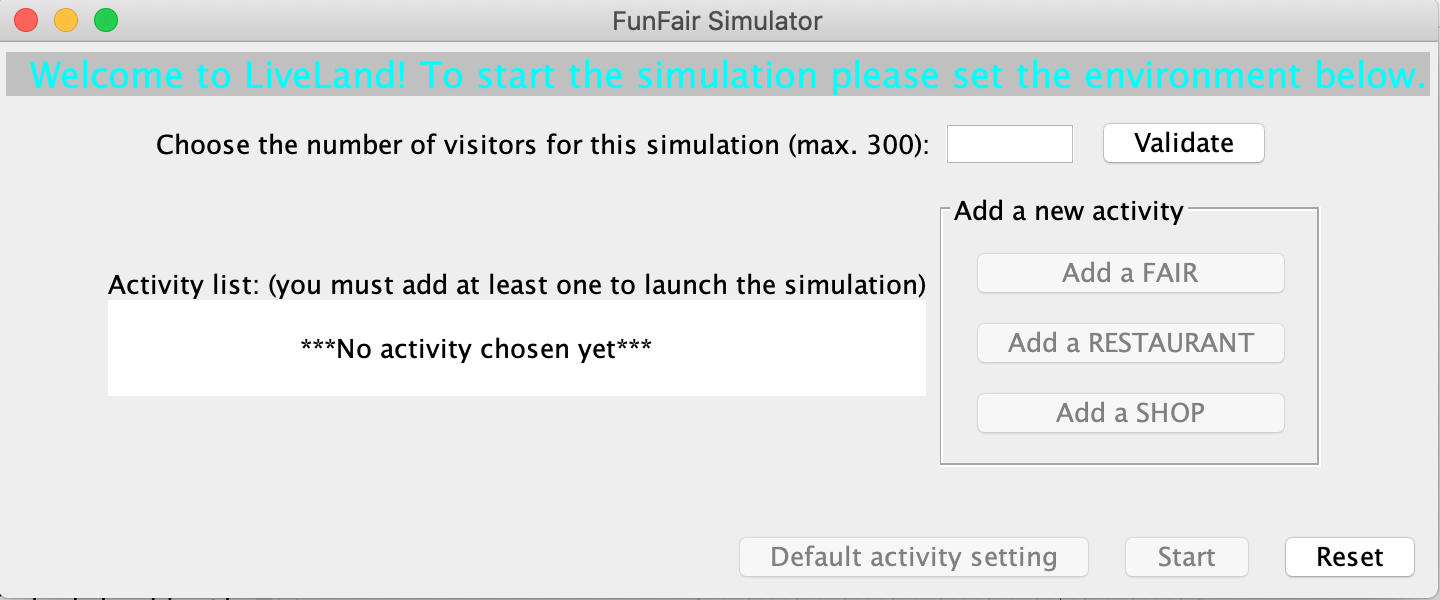
\includegraphics[width=.7\textwidth]{OOP-LiveLand/img/01- Pannello iniziale.png}
\label{img:menu}
\end{figure}

\paragraph{}Dopo aver validato il numero, che deve essere compreso tra 1 e 300, si decide se inserire manualmente le giostre, i ristoranti e i negozi e i loro corrispettivi nomi oppure se usare le attività di default proposte.
Se si sceglie di inserire manualmente apparirà questa nuova finestra dove si sceglie tra la giostra per adulti o quella per bambini, il nome e la capienza.

\begin{figure}[h]
\centering{}
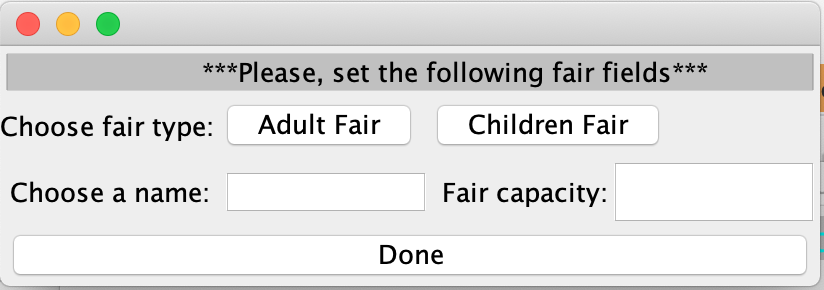
\includegraphics[width=.7\textwidth]{OOP-LiveLand/img/02- paneelo inserimento giostre.png}
\label{img:fair}
\end{figure}

\paragraph{\\}Dopo aver premuto il tasto “done” si potrà decidere di aggiungere altre giostre oppure di proseguire con l’inserimento delle attività. 

\begin{figure}[h]
\centering{}
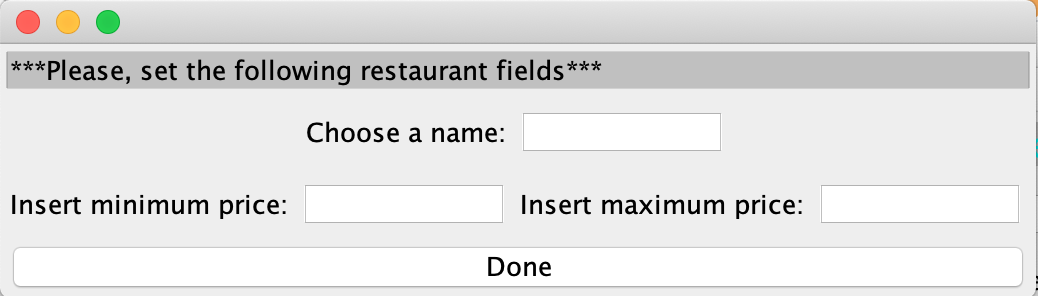
\includegraphics[width=.7\textwidth]{OOP-LiveLand/img/03-panello inserimento ristorante e shop.png}
\label{img:profit}
\end{figure}

\paragraph{\\\\}Nell’inserimento dei ristoranti e delle giostre si attribuisce il nome, il prezzo minimo e massimo che una persona può spendere all’interno di essi.
Quando l’utente finirà di aggiungere ciascuna attività apparirà nella finestra principale la lista delle attività in cui saranno elencate le scelte effettuate con i corrispettivi nomi.

\begin{figure}[h]
\centering{}
\includegraphics[width=.7\textwidth]{OOP-LiveLand/img/04-Dove vengono visualizzate le attività.png}
\label{img:attività}
\end{figure}

\onecolumn
\paragraph{}Dopo aver creato almeno un’attività è possibile avviare la simulazione premendo il pulsante “start”. Si consiglia di lasciar scorrere la simulazione grafica per un tempo di almeno 20/30 secondi per poter ottendere risultati coerenti.

\begin{figure}[h]
\centering{}
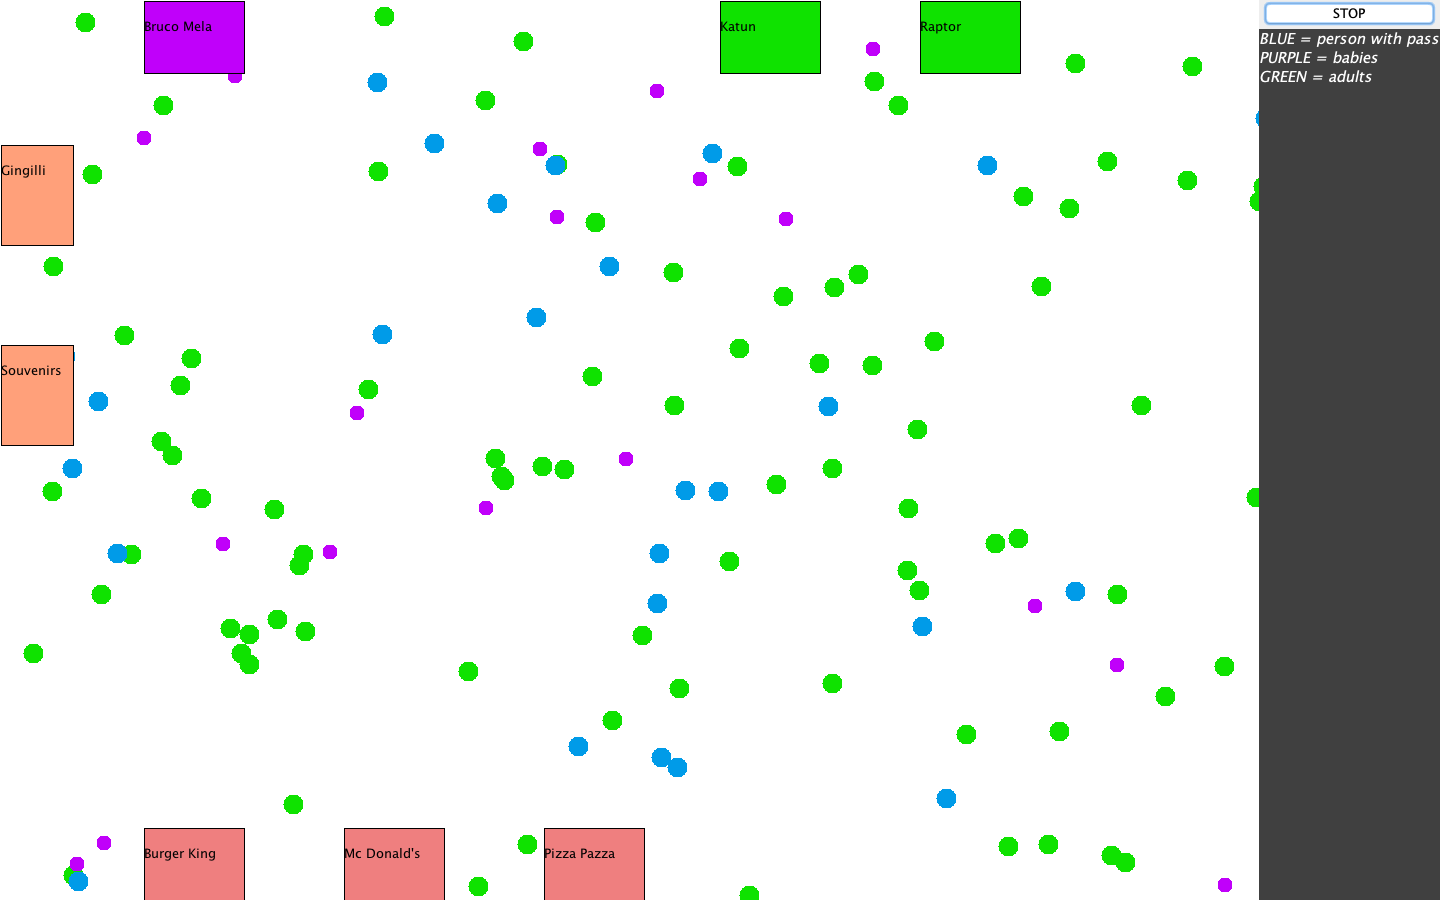
\includegraphics[width=.6\textwidth]{OOP-LiveLand/img/05 - simulazione .png}
\label{img:simulazione}
\end{figure}

\paragraph{\\}Durante la simulazione è possibile interromperla del tutto con il pulsante “stop” il quale farà apparire le statistiche finali con i grafici i quali potranno essere salvati su file mediante l'apposito menu a tendina "Save Analysis".

\begin{figure}[h]
\centering{}
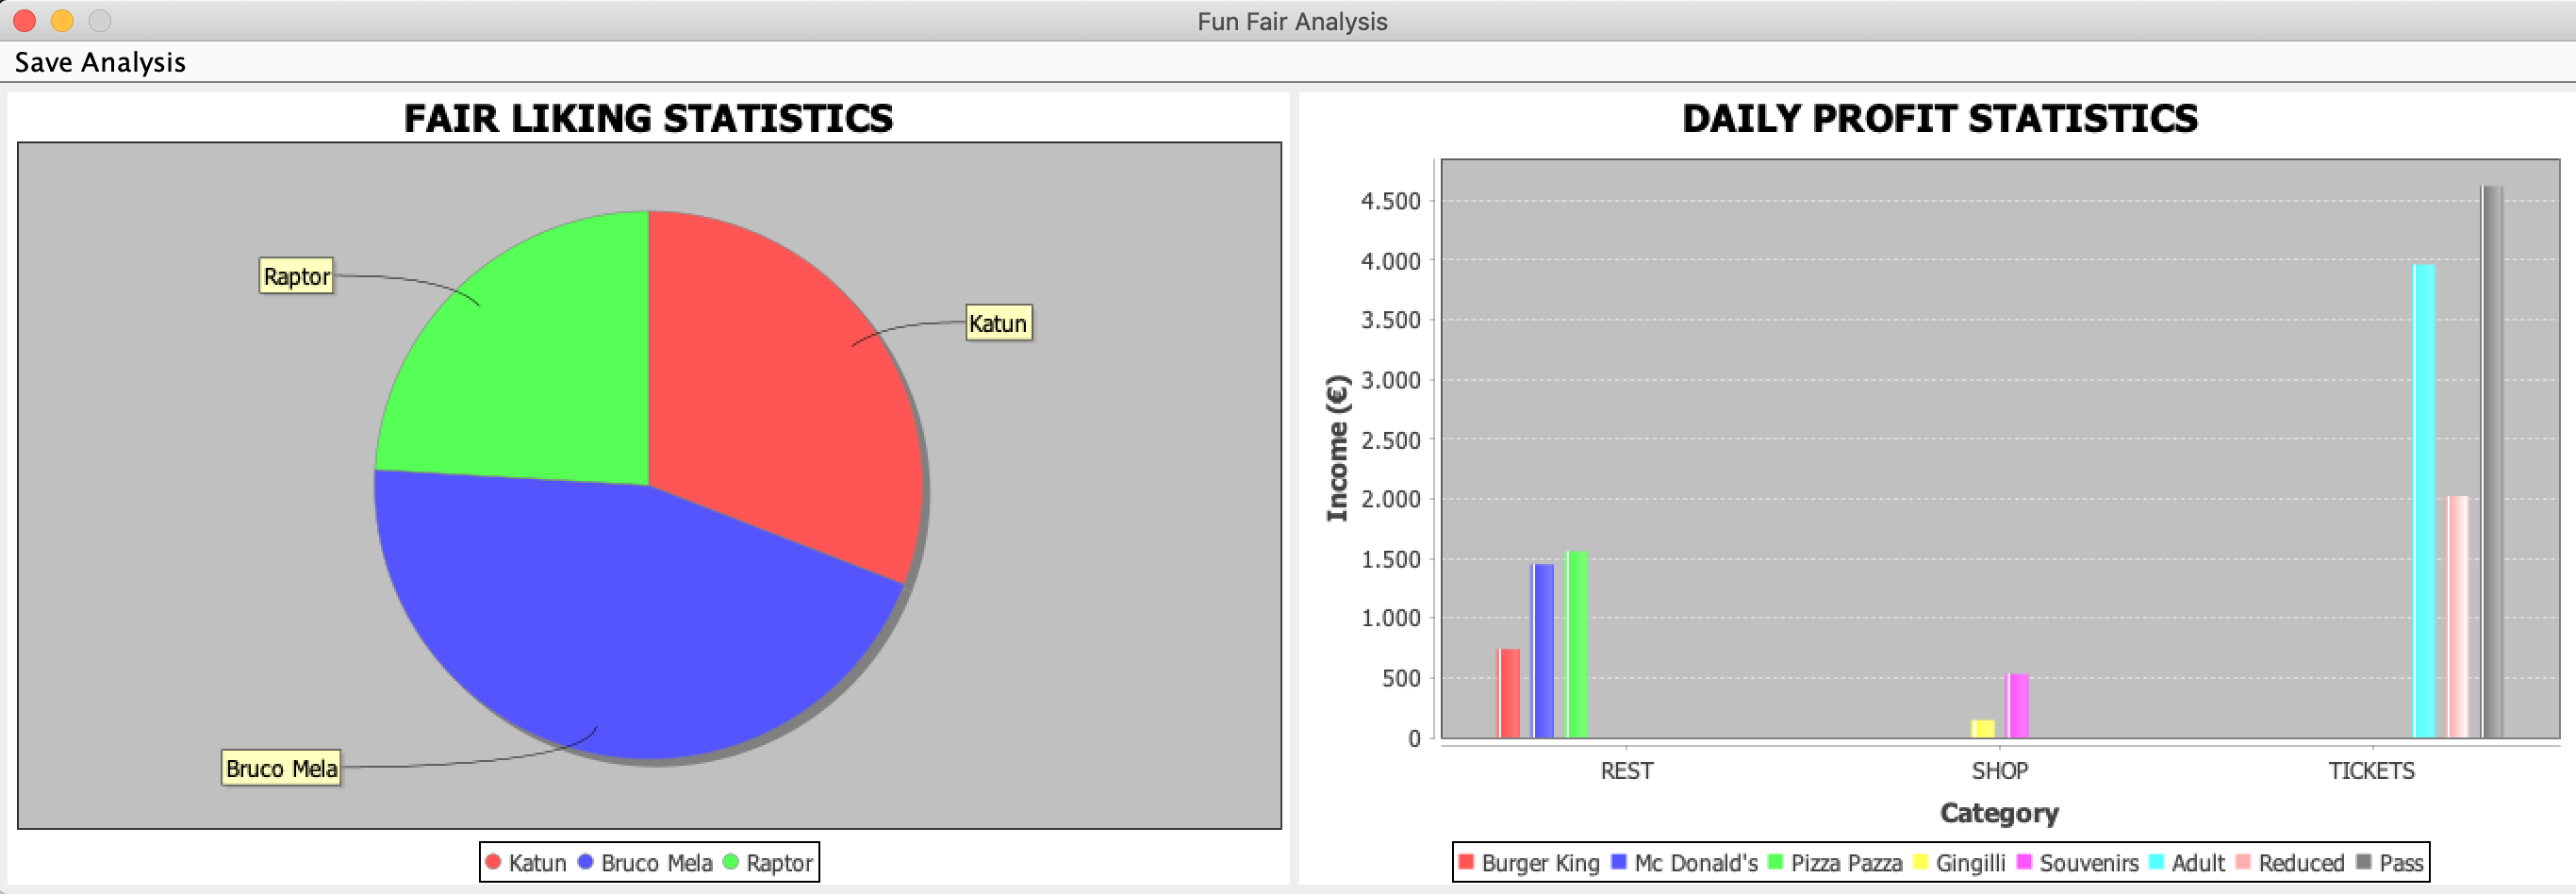
\includegraphics[width=.95\textwidth]{OOP-LiveLand/img/06-Analisi.png}
\label{img:analisi}
\end{figure}

Si segnala che qualora si desiderasse salvare l'analisi prodotta, si può scegliere il file su cui salvare una rappresentazione testuale dei dati ottenuti, oppure salvare su un file di default, che si troverà nella home directory con nome "output.txt". Inoltre, si ha anche la possibilità di salvare le statistiche ottenute come immagine in formato jpeg, che saranno automaticamente salvate nella home directory dell'utente con i nomi "LiveLandFairPieChart" e "LiveLandProfitBarChart".


\chapter{Bibliografia}
\bibliographystyle{alpha}
\bibliography{13-template copia}
Il presente documento è stato redatto in Latex sulla base del template fornito dal docente D. Pianini in laboratorio.

\end{document}